\usepackage{lipsum}
\usepackage[automake,toc]{glossaries}
\usepackage{caption}
\usepackage{listings}
\usepackage{xcolor}
\usepackage{filecontents}
\makeglossaries
% Term definitions 

\begin{document}

% =======================================================================================
%\cleardoublepage % Forces the first chapter to start on an odd page so it's on the right

% =======================================================================================
%                                   PREAMBLE
% =======================================================================================
\coverpage{\TITLE}{\SUBTITLE}{\AUTHOR}{\DATE}{\SUBJECT}
%----------------------------------------------------------------------------------------
\newpage
\tableofcontents

% =======================================================================================
%                                   PART I
% =======================================================================================
\part{Introduction to Cardano Smart Contracts}
%----------------------------------------------------------------------------------------
\newpage
\chapter{Overview of Cardano Blockchain} \label{ch:overview}
\subsection{History} \label{sec:overview}

Charles Hoskinson, along with Jeremy Wood, co-founded Cardano, both were part of Ethereum before. In 2015, they established Input Output Hong Kong to create and develop more sustainable blockchain solutions. Utilizing a peer-reviewed approach to blockchain development and introducing a novel consensus mechanism called \textbf{Ouroboros}, Cardano was prepared for its Mainnet launch in 2017.

\subsection{Ouroboros}

Ouroboros relies on a \textbf{proof of stake} consensus. Rather than requiring nodes to engage in computationally intensive work as in PoW chains, nodes are randomly selected based on the amount of ADA they hold at stake. This approach serves two purposes: it is more energy-efficient and incentivizes nodes to act responsibly as their stake is at risk in case of misbehavior.

\subsection{Cardano Architecture}

The blockchain model comprises several components. Users interact with the current ledger state by creating transactions, which are then submitted to the mempool until they are included in a block. Blocks are mined by stake pools, which are rewarded for their efforts and share these rewards with their delegators. Increased decentralization is achieved with more stake pool operators.
\subsection{Improvements from Other Blockchains}

Cardano offers several advantages over other chains:

\begin{itemize}
  \item \textbf{\textit{\gls{Determinism}}}: This feature enables transaction chaining.
  \item \textbf{Predictable Fees}: There is no risk of pending transactions due to fee increases.
  \item \textbf{Sustainability}: Unlike PoW, which is power-intensive, Cardano's approach is more sustainable.
  \item \textbf{Native Tokens}: Tokens are stored on the ledger, allowing smart contracts to interact with them. Users have control over tokens in their wallets, which cannot be frozen by external parties.
\end{itemize}

Scaling is currently the most significant challenge for the ecosystem. The ability to handle high volumes of users without being limited by block or transaction size is crucial for increasing adoption.

\subsection{\textit{Determinism} and predictable fees to make a better user experience}
Why \textbf{\textit{Determinism}} is important in smart contract programming?
Cardano inherits determinism from Bitcoin, once all the fields of a transaction are decided you will always get the same transaction Hash.
But more importantly, if you can get the hash of a transaction before actually submitting, you can even create a following transaction, relying on the first one.
This is usually called transaction chaining, I can create a chain of transactions that are not submitted, and this can allow me to speed up the user flow.
Ok, let's try to simplify even more this concept.
\begin{itemize}
  \item Alice, Bob and Raul are in a Bar, each has 100 ADA
  \item Alice sends to Raul 50 ADA but the blockchain right now is super clogged
  \item However Raul is already able to build a transaction to send 120 ADA to Bob because even if the blockchain is clogged, the hash of the transaction is already decided and won't change at all
  \item Now even Bob can send 220 ADA to someone else, even before the transactions are confirmed, due to Cardano determinism he can use transactions that are not confirmed yet
\end{itemize}

Everything seems amazing, perfect. Where is the issue?
What happens if for some reason Alice had her transaction with a deadline of 1 hour?
In that case, Alice's transaction could never become valid, therefore every other transaction depending on that will never make it.
This means that everything goes to the beginning, Alice, Bob and Raul have 100 ADA each. This is a problem if each of them paid for goods in the real world and now they get their money back.

Why do predictable fees matter and what's their role in \textit{determinism}?

On Bitcoin when you set inputs (what you spend), outputs (who gets the money) and fees you can get the transaction hash.
This happens also on Cardano, however on Bitcoin, there is a fee market, therefore the fees you set may not be enough to cover the cost of having the transaction in the next blocks.
So on Bitcoin fees may need to change, there is an RBF feature that allows you to speed up a transaction increasing the fee cost.
But this also leads to a change in the transaction hash, therefore we can't always build a chain of transactions on Bitcoin because one transaction could change, making all the following invalid.

On Cardano there is no fee market, in this way, once you pay enough to cover the processing costs, that transaction will be in the following blocks. Fees are not dynamic and can't change.

Even if it sounds cool, this leads to a problem, if there is no way of speeding up my transaction or making it possible to get priority over others, how can a protocol that needs instant settlement work?
This is an open question that lately has been discussed as a tier fee market on Cardano.

\newpage


\section{Importance and Applications of Smart Contracts}

Smart contracts are a concept born alongside Ethereum, enabling the execution of code and interactions without a third party. Once initiated, the terms of the contract are set by the parties involved, and no one can stop or interfere thereafter.

However, history teaches us that some protocols have included backdoors within their smart contracts, leading to fund theft or enabling bad actors to access users' funds.

Let's start with the basics.

\subsection{What is a Smart Contract?}

A smart contract is a decentralized software accessible to users on the blockchain, typically through a website interface. Users interacting with the contract can perform operations (financial, trading, storage) without requiring permission from a third party.

The essential components of a smart contract are:

\begin{itemize}
  \item \textbf{Parties}: Who can interact with the contract? Is it open to everyone, specific users, or owners of particular assets?
  \item \textbf{Actions}: What operations can users perform with the contract? These could include depositing funds, creating NFTs, storing data, reading data, withdrawing funds, and more.
  \item \textbf{Rules}: Define the actions each party can take under specific conditions.
  \item \textbf{Data Fields}: What data is involved in interactions with the contract, and how can each step of the interaction be tracked?
\end{itemize}
\subsection{Applications}

In a typical decentralized exchange (DEX) application, the parties are liquidity providers and traders. Liquidity providers can deposit and withdraw liquidity, while traders can only perform swaps. Rules dictate that liquidity providers must hold LP tokens in their wallets, while traders must have sufficient funds to cover transactions. Data fields stored in the contract typically include LP tokens, fees for liquidity providers, and token data.

In a marketplace scenario, the parties are sellers and buyers. Sellers can sell assets, while buyers can buy them. Rules stipulate that sellers must possess the assets they intend to sell, and buyers must have sufficient funds to purchase assets and pay sellers. Data stored includes the seller's address, payment amounts, royalties (if applicable), and platform fees.

On Cardano, specific actions might include \textbf{\textit{Cancel Listing}} and \textbf{\textit{Buy}}. \textbf{\textit{Selling/List}} is more of a smart contract interaction than an action.

\begin{remark}
  A smart contract action involves a transaction where the smart contract is invoked in the inputs. If the smart contract is present only in the outputs, it's considered a smart contract interaction.
\end{remark}

There can be many more smart contract applications, imagination is the limit, and some applications may work better on Cardano due to UTXO architecture or on EVM chains due to the account model.
Let's consider the case of a dex, it can be either \textbf{\textit{\gls{orderbook}}} or \textbf{\textit{\gls{AMM}}}. The orderbook works perfectly in a UTXO blockchain because every order can be a single UTXO.
While on EVM chains orderbook dexes struggle because they are limited by the memory of the smart contract.
On the opposite side, building an AMM on Cardano requires a lot of emulation, since the pool is a single UTXO, more parties can't spend it at the same time, that's why we found as solutions the batchers.
Batchers match the orders with the single UTXO liquidity pool.
This concept is not efficient however AMM are more user-friendly usually and that's why currently Cardano is the one leading in liquidity volumes.

\subsection{Smart Contract audits}

Once a smart contract is developed and ready to launch an audit should be done, this is to ensure that the code is safe and no issues may arise once people start interacting with it.
Audits play a critical role in the deployment of smart contracts, serving as a crucial safeguard against potential vulnerabilities and ensuring the integrity of the code.
Smart contracts, being immutable, leave little room for error once deployed, making thorough scrutiny prior to launch imperative.
Audits help identify security flaws, logic errors, and vulnerabilities that may compromise the contract's functionality or jeopardize users' funds.
By subjecting the code to rigorous review by experienced professionals, audits instill confidence among users and investors, fostering trust in the decentralized ecosystem. Moreover, audits contribute to the overall maturation of the blockchain space, driving standards for secure coding practices and enhancing the reliability of smart contract applications.
Ultimately, investing in audits upfront mitigates the risk of costly exploits or breaches down the line, safeguarding both the project's reputation and the interests of its stakeholders.

But audits have a cost and sometimes early projects may not afford that much.

Opensource can be a way in order to launch a project asking for external reviews coming from the community, usually bug bounty programs are run in order to incentivize users to collaborate in the task of finding risks in the smart contract code.

\subsection{Smart Contract risks}

On Cardano there are some risks regarding smart contracts that we'll study better in the following chapters, but here are a few of them as a preview:

\begin{itemize}
  \item Double satisfaction attack: User may spend two inputs that require similar conditions
  \item Dust attack: Users may add spam tokens in a smart contract making it impossible to retrieve funds from it
  \item Spam Contract: A second smart contract can run together with the attacked one, making it possible to unlock funds from the first
  \item Datum attack: A datum of the contract may be corrupted making unspendable the funds inside the contract
  \item backdoor: All the funds of the contract may be retrieved by someone who coded a backdoor
\end{itemize}

\subsection{The cost of deploying a contract}

Deploying a contract onto the blockchain carries no direct cost, allowing widespread accessibility. However, it's essential to consider additional expenses, especially if utilizing reference scripts like ADA, which may necessitate funds for storage on the blockchain. Moreover, while users typically prefer interacting with contracts via frontends, developing and maintaining such interfaces entail both frontend and backend costs. It's imperative to conduct thorough economic assessments before project launch, ensuring expenses don't surpass revenues. Abruptly discontinuing services without prior notice could result in users losing their funds, highlighting the importance of transparent communication in managing smart contract projects.
\section{Advantages of Cardano for Smart Contract Development}

Two years ago, if you asked me about the advantages of writing smart contracts on Cardano, I would have struggled to answer. However, now I can easily list several:

\begin{itemize}
  \item \textbf{\gls{Composability}}: The ability to create a transaction involving multiple contracts and perform actions with each of them.
  \item \textbf{User-Friendly}: No longer requiring Haskell, languages like Aiken, Opshin, and more offer a user-friendly experience.
  \item \textbf{\gls{Liquid Staking}}: Thanks to Cardano staking, smart contracts can delegate ADA or keep funds staked with liquidity providers.
  \item \textbf{UTxO Skills}: While much of the focus has been on Ethereum Virtual Machine (EVM) smart contracts, the UTXO model is ideal for solutions like ZK rollups, as it's easier to implement compared to the account model.
\end{itemize}

If you're still interested in becoming a Cardano smart contract wizard after this introduction, we can continue in the next chapter, where we'll install the components needed to \textbf{build on Cardano}.

% =======================================================================================
%                                   PART II
% =======================================================================================
\part{Setting Up the Development Environment}
%----------------------------------------------------------------------------------------
\newpage
\chapter{Installing and Configuring Cardano Development Tools} \label{ch:setup}
\section{Installing and Configuring Cardano Development Tools}\label{sec:setup}
The purpose of this book is to gather all the information for developing Cardano that currently is scattered around.
What are we going to use for our project?


\begin{itemize}
    \item \textbf{A hot Wallet}: We are going to use a wallet to test our contracts, this wallet will be used to receive tADA. We'll never store our main ADA holdings in this wallet: Wallets recommended for testnet are Nami on desktop and  Vespr for mobile.
    \item \textbf{A indexer account}: Indexers are the ones that will provide us the APIs in order to interact with the chain, we won't need to run a node for testing, let's use services and projects already there like \textbf{Maestro}, let's set up an account and get the API key.
    \item \textbf{Lucid library}: Lucid is not maintained anymore as a function and has been replaced by COMING SOON, however for testing and understanding the flow of Cardano transactions it can be really useful.
    \item \textbf{tADA}: How are we going to test without having testnet ADA? let's not mess up real ADA
    \item  \textbf{IDE}: Personally I use Visual Studio Code as IDE, but any other editor is ok since we are going to 
    \item \textbf{Cardano Node:} This is NOT mandatory at all, as homework, we could try to set up a Cardano node and interact with the chain using cardano-cli (command line), however, this is something we can do in our free time, there are other hobbies out there better than this, swimming, dancing or reading a book.
\end{itemize}

\section{Hot wallets on Cardano}
When it comes to the wallet choice on Cardano the question we should ask ourselves is: Desktop or Mobile?

\begin{table}[h!]
    \caption{Current Cardano wallets available, updated in Q2 24}
    \begin{tabular}{llll}
    Wallets & Desktop & Mobile & Website                    \\
    Nami    & X       &        & https://www.namiwallet.io/ \\
    Eternl  & X       & X      & https://eternl.io/         \\
    Begin   &         & X      & https://begin.is/          \\
    Vespr   &         & X      & https://vespr.xyz/         \\
    Lace    & X       &        & https://www.lace.io/       \\
    NuFi    & X       &        & https://nu.fi/             \\
    Yoroi   & X       & X      & https://yoroi-wallet.com/  \\
    Flint   & X       & X      & https://flint-wallet.com/  \\
    Gero    & X       &        & https://www.gerowallet.io/ \\
    Typhon  & X       &        & https://typhonwallet.io/   \\
    \end{tabular}
\end{table}

Test the wallet you like most and pick the one that gives you more user-friendly vibes for your use, a developer may require a very detailed wallet, however, a basic user may need just some very simple buttons without details.

\section{Setting Up and Connecting to Cardano Testnet}
So let's install a wallet and config for testnet 

In this example, we'll install the Nami wallet that we can find \href{https://www.namiwallet.io/}{here}

Once we install the wallet we'll get 24 seed phrase words

\begin{remark}
Never share the seedphrase or store it on a cloud, use paper or different ways to store it, software can keep track of your seedphrase and you could lose the funds.
\end{remark}

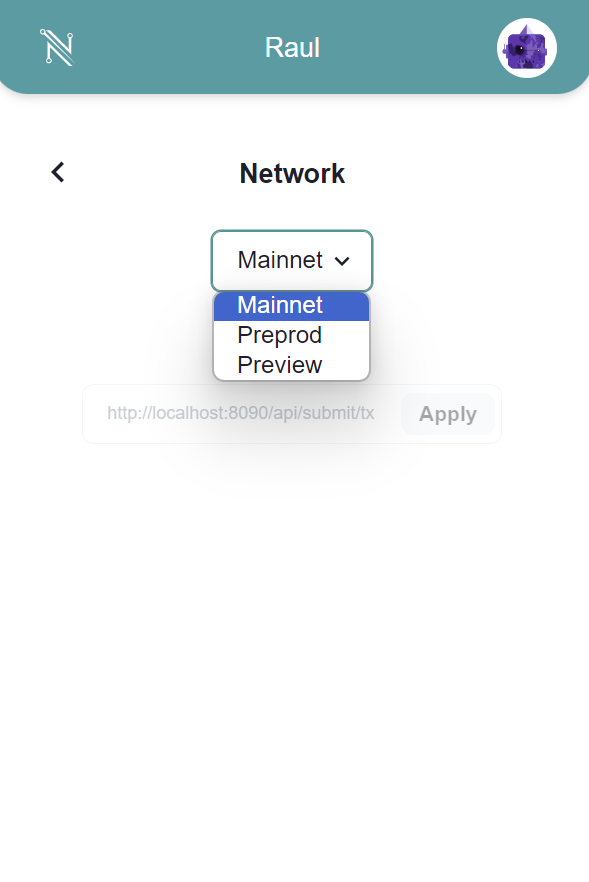
\includegraphics{wallet_preview}

Let's set Nami to \textbf{testnet preview} and we'll finally get our wallet in testnet 

\subsection{Preview and Preprod testnets}

\begin{itemize}
    \item \textbf{Mainnet}: This is the live network where real transactions occur using actual ADA. It's the primary arena where users engage with Cardano wallets, exchanges, and decentralized applications (dApps).
    \item \textbf{Preprod}: Acting as a staging ground for major upgrades and releases, Preprod is a testing environment where developers validate changes before deploying them to the mainnet. Utilizing test ADA acquired from the faucet, developers simulate real-world scenarios, ensuring everything functions as intended before the changes go live. Preprod typically mirrors mainnet's structure, forking nearly simultaneously to ensure alignment.
    \item \textbf{Preview}: Serving as a testing environment to showcase upcoming features and functionality, Preview allows developers and users to explore and provide feedback on new developments before they reach the wider community. Like Preprod, test ADA from the faucet facilitates testing. Notably, Preview precedes mainnet hard forks by a minimum of four weeks, offering ample time for thorough evaluation and refinement based on community input.
\end{itemize}

\subsection{Get tADA}

In order to receive tADA we can use the official faucet from Cardano at the following \href{https://docs.cardano.org/cardano-testnets/tools/faucet/}{link}

The process doesn't involve any payment and at the end of your testing, ideally, you should return tADA back so other devs can work with it.

\subsection{CIP30}

To connect our wallet with any webpage we'll use \gls{CIP}30 reference, we can find the list of methods to connect and invoke the functions of the wallets at this \href{https://www.cardano-caniuse.io/}{page}

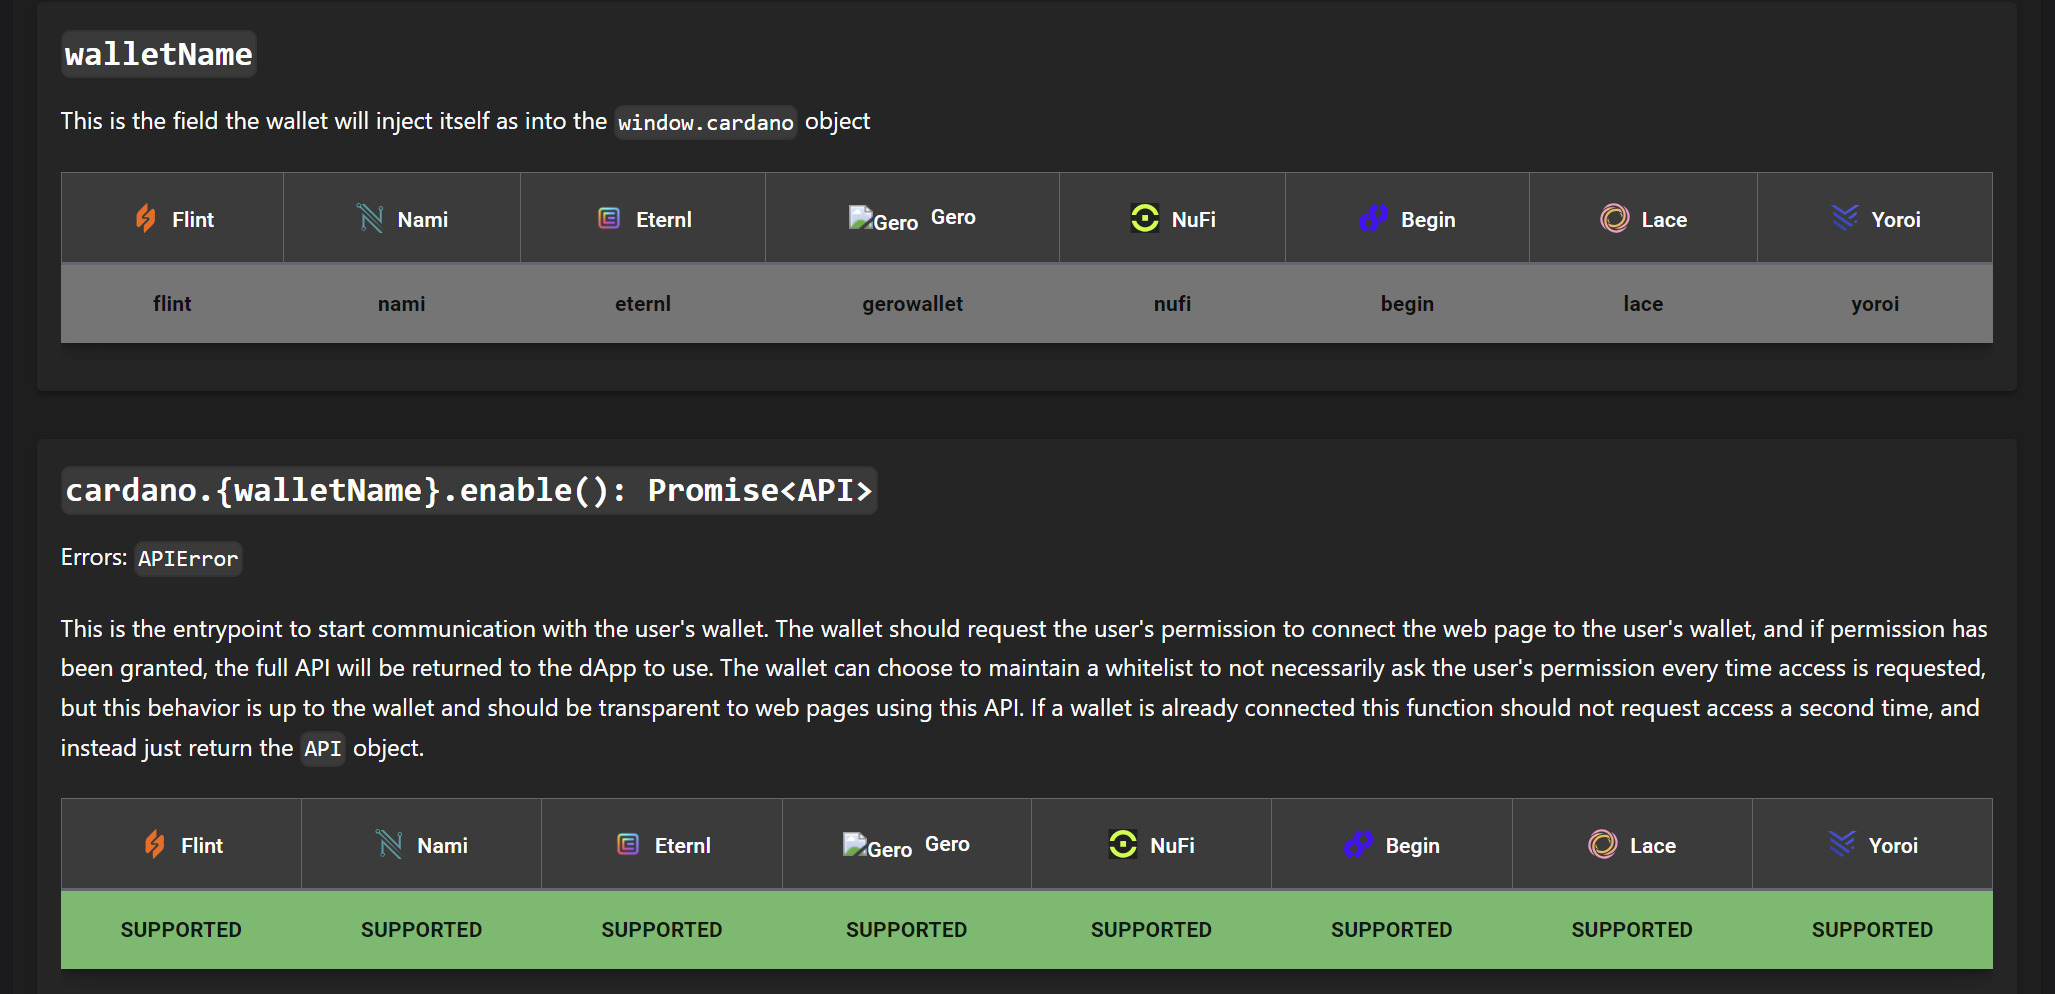
\includegraphics[scale=0.3]{cip30}

The steps to interact with a wallet following cip30 are:

\begin{itemize}
    \item \textbf{cardano.{walletName}.enable()}: we get an API object as Promise, this will create a popup message to allow the wallet to connect to the current website
    \item \textbf{api.getBalance()}: using the API object we got before, we get the total amount of Lovelace in the wallet (1 ADA = 1000,000 Lovelace)
    \item \textbf{api.signTx}: Signing a tx that was built with Lucid or any other library we sign and interact with the blockchain 
\end{itemize}

\begin{remark}
    EXERCISE 1: Create a webpage with 2 buttons, 1 to enable the wallet connection and, a second button to view the amount of ADA in the wallet.
\end{remark}




\section{Interacting with Cardano Node and Wallet APIs}

CIP30 is not enough, what if we want to get the information regarding a specific NFT in our wallet?
How to get the list of tokens inside the wallet and get information regarding their circulation supply?

We need an indexer. We could set one on our own or use a service, in this book we'll use \textbf{Maestro} as a service provider so the first thing to do is:

\subsection{Create a Maestro account}

Head over \href{https://dashboard.gomaestro.org/login}{Maestro login} page and create an account, here we'll be able to get the API keys to interact with Cardano.

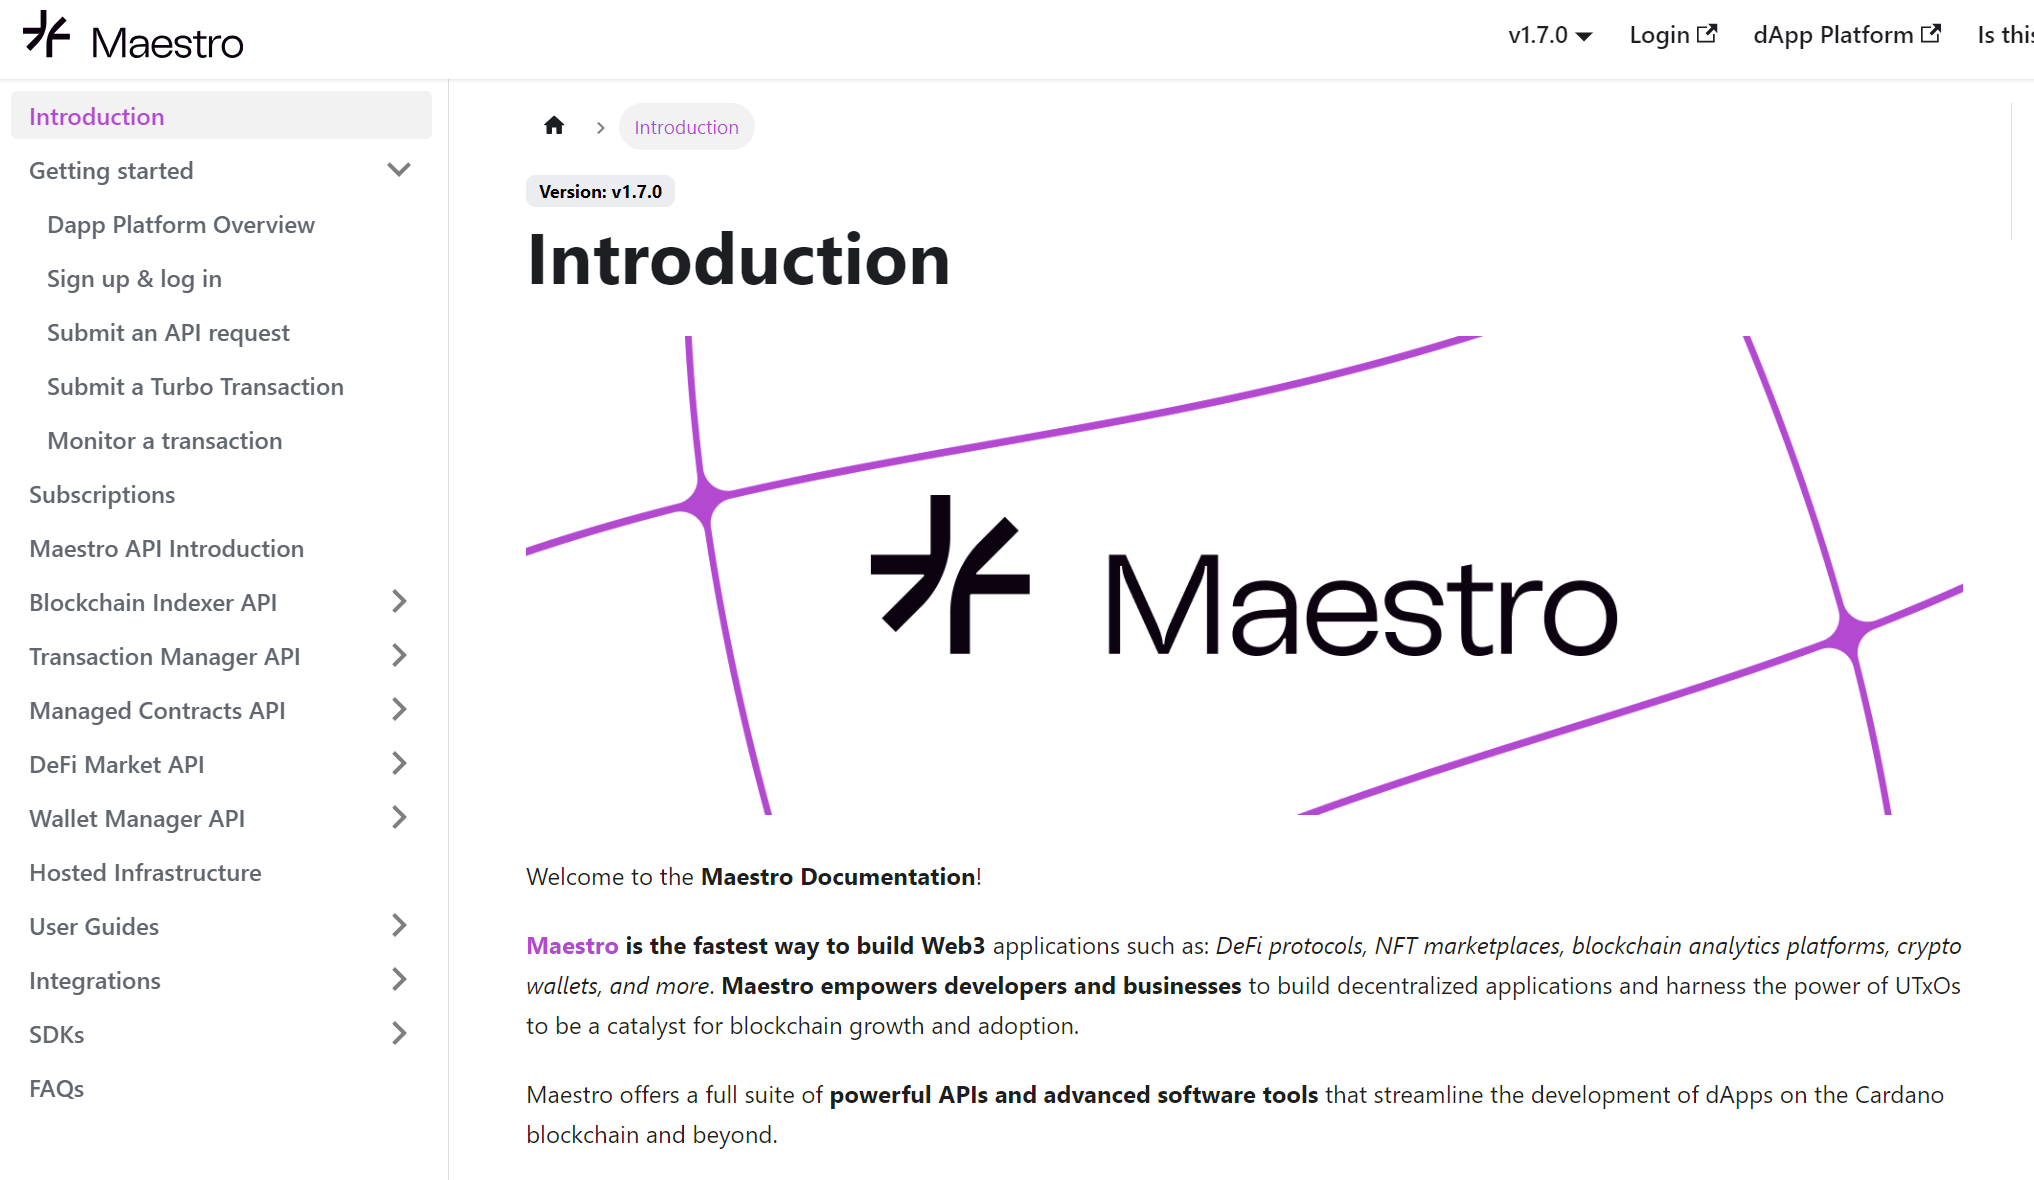
\includegraphics[scale=0.3]{maestro.png}

Maestro is going to be our key to getting all the possible APIs in order to interact with Cardano, here are the possible things we can do with these APIs:

\begin{itemize}
    \item Get the history of an address with this \href{ttps://docs.gomaestro.org/Indexer-API/Addresses/txs-by-address}{API}
    \item Get all the assets of a specific policy 
    \item Get the address holding a specific ada handle
    \item Get the history of holders for a specific NFT 
    \item and much more 
\end{itemize}

Now that we have a way to interact with a wallet and APIs to query the Cardano blockchain we are ready to put our hands on the real coding part.

\subsection{Indexer alternatives}

If you would like to explore additional API providers you should consider the following:

\begin{itemize}
    \item Blockfrost: The very first API provider for Cardano \href{https://blockfrost.io/dashboard}{link}
    \item Kupo: A tool that requires a node in order to host your own11 indexer \href{https://github.com/CardanoSolutions/kupo}{Github}
    \item Db-sync: Additional indexer that requires a Cardano Node, this is the very first one that was created \href{https://github.com/IntersectMBO/cardano-db-sync}{Github}
\end{itemize}

Now Let's code smart contracts.

\begin{remark}
    EXERCISE 2: Head over to http://cnftlab.party/ and connect your testnet wallet, mint a collection of NFTs and then use Maestro to get the information of each NFT of your collection.
\end{remark}


\section{Setting Up a Cardano Node on Contabo Cloud VPS}

\subsection{Step 1: Provisioning a Contabo Cloud VPS}
\begin{enumerate}
    \item Sign up for a Contabo Cloud VPS plan, such as the "Cloud VPS L".
    \item Once you have access to your VPS, log in via SSH.
\end{enumerate}

\subsection{Step 2: Downloading and Extracting Cardano Node Software}
\begin{enumerate}
    \item Navigate to the official Cardano GitHub release page: \href{https://github.com/input-output-hk/cardano-node/releases/tag/8.1.2}{Cardano Node Releases}.
    \item Download the Cardano Node software for macOS by running the following command:
    \begin{verbatim}
    wget https://github.com/input-output-hk/cardano-node/releases/download/8.1.2/cardano-node-8.1.2-macos.tar.gz
    \end{verbatim}
    \item After the download completes, create a directory named "node" and extract the downloaded files into it:
    \begin{verbatim}
    mkdir node
    tar xvzf cardano-node-8.1.2-macos.tar.gz -C node
    \end{verbatim}
\end{enumerate}

\subsection{Step 3: Setting Up Node Configuration}
\begin{enumerate}
    \item Create the necessary directories:
    \begin{verbatim}
    cd node
    mkdir mainnet
    cd ..
    mkdir sockets
    \end{verbatim}
    \item Create a systemd service file for the Cardano Node:
    \begin{verbatim}
    sudo nano /etc/systemd/system/cardano-node.service
    \end{verbatim}
    
    Paste the following content in the file:

    \begin{verbatim}
sudo nano /etc/systemd/system/cardano-node.service
Now we should copy and paste the following lines:
[Unit]
Description=Cardano Pool
After=multi-user.target
[Service]
Type=simple
ExecStart=/home/ubuntu/nodev30/cardano-node run --config
/home/ubuntu/nodev30/config/mainnet-config.json --topology
/home/ubuntu/nodev30/config/mainnet-topology.json --database-path
/home/ubuntu/nodev30/mainnet/db/ --socket-path  /home/ubuntu/nodev30/sockets/node.socket --
host-addr 0.0.0.0 --port 3001

KillSignal = SIGINT
RestartKillSignal = SIGINT
StandardOutput=syslog
StandardError=syslog
SyslogIdentifier=cardano
LimitNOFILE=32768

Restart=on-failure
RestartSec=15s
WorkingDirectory=~
User=USERNAMEVPS

[Install]
WantedBy=multi-user.target
    \end{verbatim}

    Save the file and exit the editor.
\end{enumerate}

\subsection{Step 4: Installing Required Dependencies and Syncing the Blockchain}
\begin{enumerate}
    \item Update package list and install necessary tools:
    \begin{verbatim}
    sudo apt update && sudo apt install liblz4-tool jq curl
    \end{verbatim}
    \item Fetch the latest blockchain snapshot and sync the blockchain:
    \begin{verbatim}
    curl -o - https://downloads.csnapshots.io/snapshots/mainnet/$(curl -s https://downloads.csnapshots.io/snapshots/mainnet/mainnet-db-snapshot.json| jq -r .[].file_name ) | lz4 -c -d - | tar -x -C /root/node/mainnet/
    \end{verbatim}
    This process may take around 30 minutes.
\end{enumerate}

\subsection{Step 5: Starting the Cardano Node}
\begin{enumerate}
    \item Enable and start the Cardano Node service:
    \begin{verbatim}
    sudo systemctl enable cardano-node.service
    sudo systemctl start cardano-node.service
    \end{verbatim}
    \item Monitor the node's status:
    \begin{verbatim}
    journalctl -u cardano-node.service -f -o cat
    \end{verbatim}
\end{enumerate}

\subsection{Step 6: Setting Up Cardano Submit API}
\begin{enumerate}
    \item Navigate to the node directory:
    \begin{verbatim}
    cd node
    \end{verbatim}
    \item Create a configuration file for the transaction submission API:
    \begin{verbatim}
    nano tx-submit-mainnet-config.yaml
    \end{verbatim}
    Paste the content from \href{https://github.com/input-output-hk/cardano-node/blob/master/cardano-submit-api/config/tx-submit-mainnet-config.yaml}{Cardano Node GitHub} into this file. Save and exit the editor.
    \item Run the Cardano Submit API with the provided configuration:
    \begin{verbatim}
    ./cardano-submit-api --tx-submit-mainnet-config.yaml --socket-path /root/node/sockets/socket node.socket --port 8090 --mainnet --host-addr 0.0.0.0
    \end{verbatim}
\end{enumerate}

\subsection{Step 7: Accessing Transaction Submission Endpoint}
With the Cardano Submit API running, you can now send transactions using your node by accessing the following URL:
\begin{verbatim}
http://VPSIPADDRESS:8090/api/submit/tx
\end{verbatim}
Replace \texttt{VPSIPADDRESS} with the IP address of your VPS.

By following these steps, you'll have successfully set up a Cardano node on your Contabo Cloud VPS and be ready to interact with the Cardano blockchain.


% =======================================================================================
%                                   PART III
% =======================================================================================
\part{Exploring the eUTxO Model}
%----------------------------------------------------------------------------------------
\newpage
\chapter{Understanding the eUTxO Model and Its Components} \label{ch:exploring}
\section{Understanding the eUTxO Model and Its Components} \label{sec:exploring}

Two popular record-keeping models in blockchain networks are the eUTXO (Extended Unspent Transaction Output) Model used by Cardano and the Account/Balance Model employed by Ethereum. This section provides a basic understanding of these models, their differences, and their respective pros and cons.

\section{eUTXO Model}
In Cardano, each transaction spends outputs from prior transactions and generates new outputs for future transactions. All unspent transactions are stored in each fully synchronized node, giving rise to the name ``eUTXO''. A user’s wallet tracks unspent transactions associated with the user's addresses, and the wallet balance is the sum of these unspent transactions.

\subsection{Example}
1. Alice gains 12.5 ADA through staking rewards, resulting in one eUTXO of 12.5 ADA.

2. Alice sends 1 ADA to Bob. Alice’s wallet uses her eUTXO of 12.5 ADA, sending 1 ADA to Bob and receiving 11.5 ADA as a new eUTXO to a new address owned by Alice.

3. If Bob had an eUTXO of 2 ADA before step 2, his wallet now shows a balance of 3 ADA from two eUTXOs.

\subsection{Account/Balance Model}
The Account/Balance Model maintains the balance of each account as a global state. It checks that an account's balance is sufficient to cover the transaction amount.

\subsection{Example}
1. Alice gains 5 ETH through mining, recorded in the system.

2. Alice sends 1 ETH to Bob, reducing her balance to 4 ETH.

3. Bob’s balance increases by 1 ETH, so if he had 2 ETH initially, he now has 3 ETH.

\subsection{Analogies}
\begin{itemize}
    \item  \textbf{eUTXO Model}: Similar to using paper bills, where each bill (eUTXO) can be spent once, and change is returned as new eUTXOs.
    \item \textbf{Account/Balance Model}: Similar to a bank's ATM/debit card system, where the bank ensures sufficient balance before approving transactions.
\end{itemize}

\subsection{Benefits}

\subsection{eUTXO Model}
\begin{itemize}
    \item \textbf{Scalability}: Enables parallel transactions and scalability innovations.
    \item \textbf{Privacy}: Provides higher privacy, especially with new addresses for each transaction.
\end{itemize}

\subsection{Account/Balance Model}
\begin{itemize}
    \item \textbf{Simplicity}: Easier for developers of complex smart contracts requiring state information.
    \item \textbf{Efficiency}: More efficient as each transaction only validates account balance.
\end{itemize}

\subsection*{Drawbacks}
\textbf{Account/Balance Model}: Susceptible to double-spending attacks, counteracted by an incrementing nonce.

Both models have trade-offs and are chosen based on specific blockchain needs. Some blockchains, like Hyperledger, adopt eUTXO to benefit from Bitcoin's innovations.


\section{Writing Transactions and Validating Inputs and Outputs}

In this section, we'll analyze the components of a Cardano transaction and how it is built using a Cardano node and then using the Lucid library.

Let's start with the following transaction:

\href{https://preview.cexplorer.io/tx/a2fcdf32987ebb729ab8f63b377e360ececbf4805713ff559d2b69bb3c543a01}{a2fcdf32987ebb729ab8f63b377e360ececbf4805713ff559d2b69bb3c543a01}

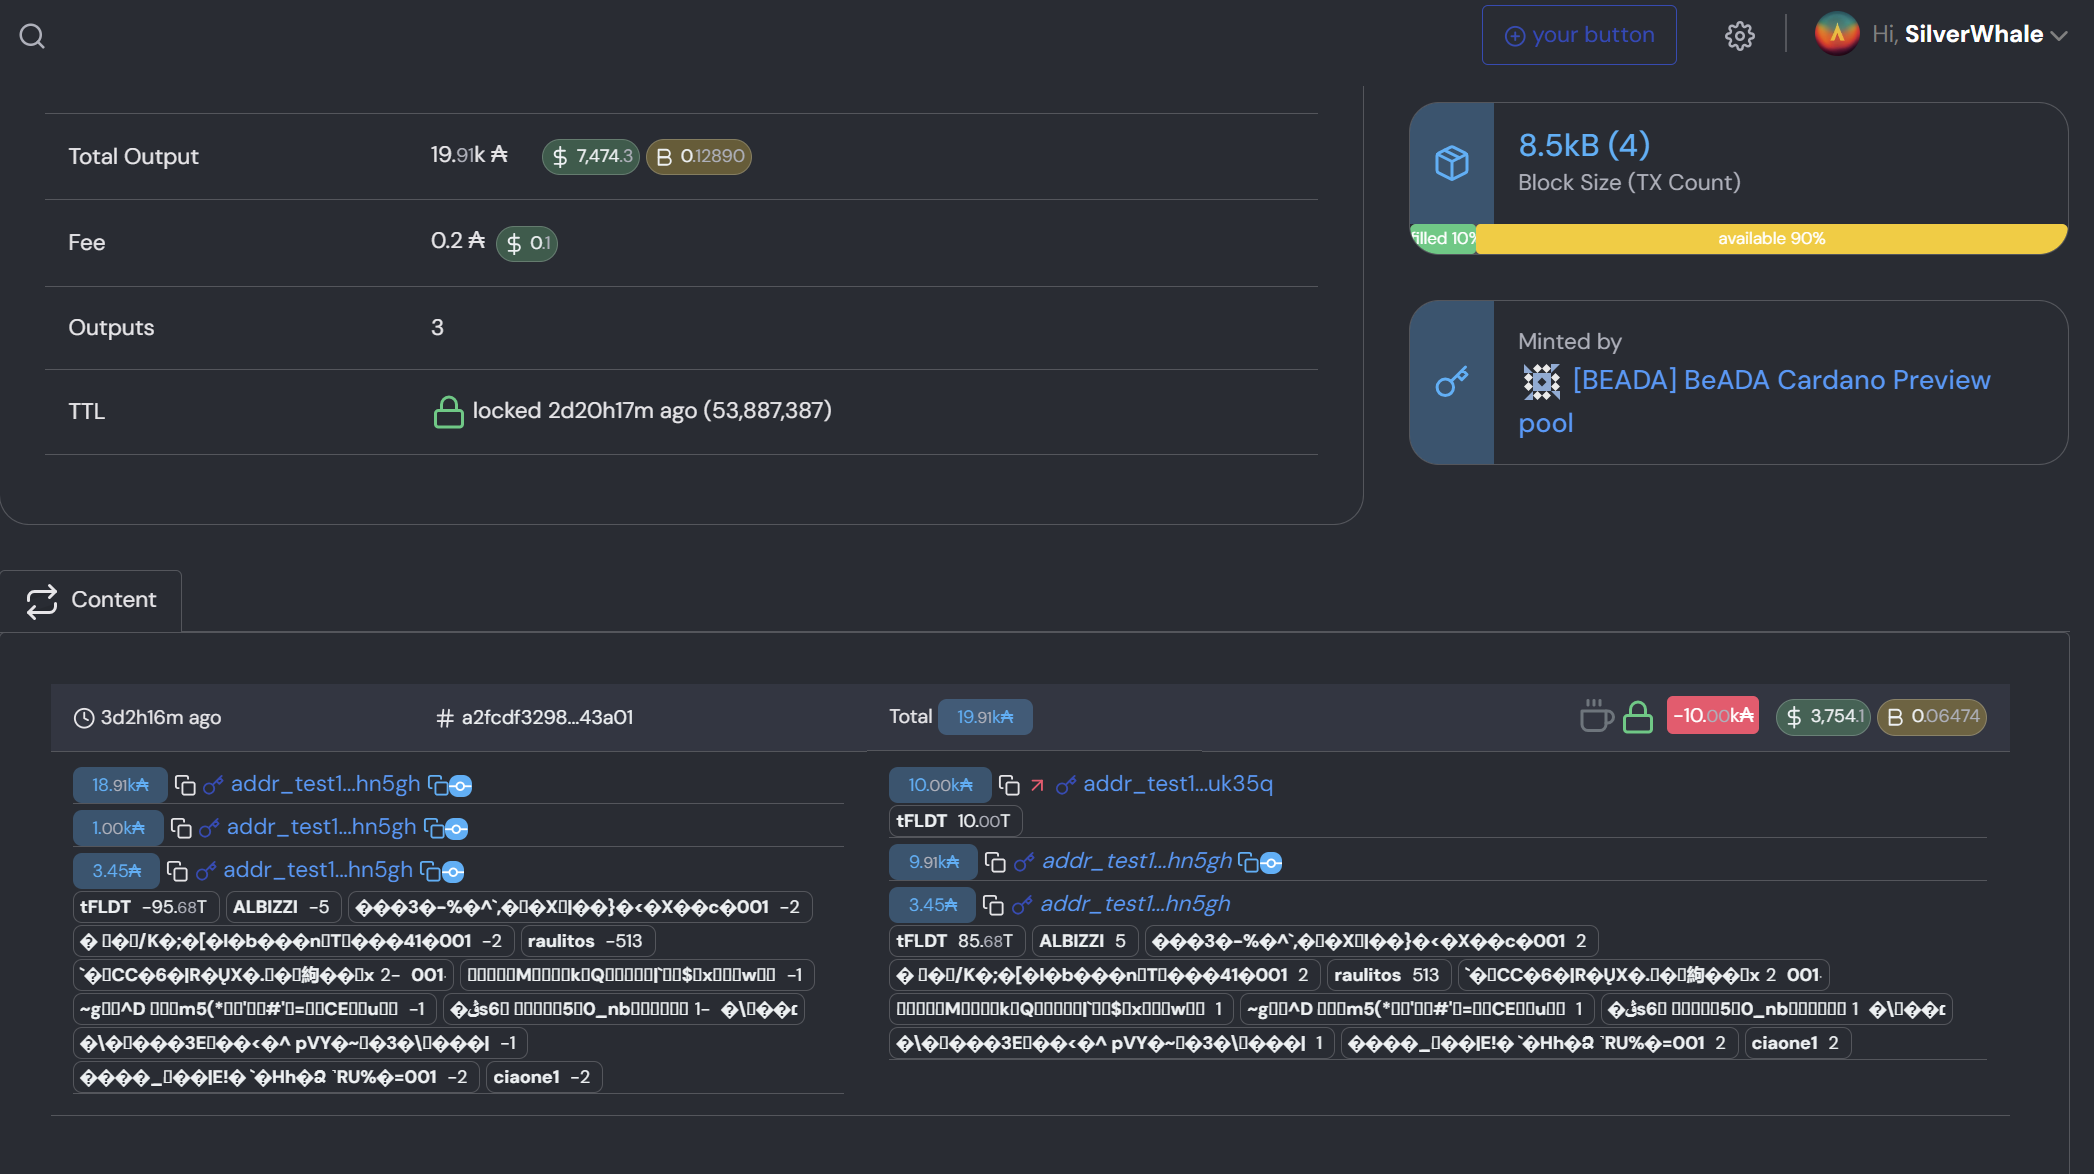
\includegraphics[scale=0.3]{transactionTestnet}

Let's analyze what we can see here:

On the \textbf{left}, we have the \gls{inputs} of the transaction. We can see that we are spending 3 inputs containing tADA and some tokens.
The inputs being spent are from the following transactions:

\begin{itemize}
    \item \texttt{5df4a4fb78650b5d8b0e761e0ade2c2ab2289b4feb97f6780b82d78b3d02bf70}
    \item \texttt{f0e29aed793164ce8192aec7ec647b7e7747206d701b0dfd4a810414f7acb96b}
    \item \texttt{5df4a4fb78650b5d8b0e761e0ade2c2ab2289b4feb97f6780b82d78b3d02bf70}
\end{itemize}

This means that for each transaction, we can obtain the transactions that generated the funds being spent directly from the hash of the inputs.
Not just this, it means that we are always able to track if the funds generated by a transaction have already been spent because they will appear as input on another transaction.

But that's not all; for each input, we are able to see from which address they come from, in this case \texttt{addr\_test1qqw...hn5gh} and also the amount of tADA and tokens that were locked inside those inputs. We'll call this \textbf{Value}.

On the \textbf{right} side, we can see the outputs of the transaction. Therefore, where is the tADA going?

We have 3 outputs:

\begin{itemize}
    \item The first output is sending 10,000 tADA and 1M tFLDT to \texttt{addr\_test1qpku...sjuk35q}.
    \item The second output is a change to \texttt{addr\_test1qqwywxe3ag9sf3jjhk8hd...fhn5gh} sending back all the tADA that was left.
    \item The third output is a change to \texttt{addr\_test1qqwywxe3ag9sf3jjhk8hd...fhn5gh} sending back all the NFTs and tokens that were leftovers.
\end{itemize}

Finally, we can see that this transaction was validated during \gls{epoch} 623, \gls{block} 2,270,567, and \gls{slot} 53,865,862.
It was confirmed by BEADA stake pool operator, and there was a 0.2 fee paid to the network.

\subsection{Build a transaction with Cardano node}

This part is not mandatory since it requires to run a Cardano node, however it is interesting to see how a transaction is built from scretch


Let's create a folder:

\begin{lstlisting}
mkdir exercise01
\end{lstlisting}

Now we create the wallet with:

\begin{lstlisting}
cardano-cli address key-gen --verification-key-file payment.vkey --signing-key-file payment.skey
\end{lstlisting}

To see the address, use the following command:

\begin{lstlisting}
cardano-cli address build --payment-verification-key-file payment.vkey --out-file payment.addr
\end{lstlisting}

And then:

\begin{lstlisting}
cat payment.addr
\end{lstlisting}

And we now see our address!

\subsection*{Checking funds in wallet}

Let's run the command:

\begin{lstlisting}
cardano-cli query utxo --address $(cat payment.addr) --mainnet
\end{lstlisting}

We will see that there are no transactions, so 0 ADA.

\subsection*{Sending funds}

Let's send some ADA to the wallet from our main wallet (try with 5 ADA) and run the command again to check the transactions:

\begin{lstlisting}
cardano-cli query utxo --address $(cat payment.addr) --mainnet
\end{lstlisting}

Now we should see some ADA. For instance, 5,000,000 lovelace means 5 ADA.

\subsection*{Check funds of any address}

If you want to check the ADA inside any wallet, the command becomes:

\begin{lstlisting}
cardano-cli query utxo --address ADDRESSTOCHECKHERE --mainnet
\end{lstlisting}

The result is all the transactions containing ADA and NFTs in the address.

\subsection*{Creating the raw transaction}

Let's copy the transaction hash that contains the 5 ADA and the index:

\begin{lstlisting}
cardano-cli transaction build-raw --fee 0 --tx-in HASHOFUNSPENTTRANSACTION#INDEX --tx-out ADDRESSRECEIVER+2000000 --tx-out $(cat payment.addr)+0 --mainnet --out-file matx.raw
\end{lstlisting}

\subsection*{Calculate the fee}

We must calculate the fee according to the network parameters that we get with the following:

\begin{lstlisting}
cardano-cli query protocol-parameters --mainnet --out-file protocol.json
\end{lstlisting}

Now:

\begin{lstlisting}
cardano-cli transaction calculate-min-fee --tx-body-file matx.raw --tx-in-count 1 --tx-out-count 2 --witness-count 1 --mainnet --protocol-params-file protocol.json
\end{lstlisting}

And we get the fee we should pay at least.

\subsection*{Build the final transaction}

Now we can finally build the complete transaction with:

\begin{lstlisting}
cardano-cli transaction build-raw --fee FEE_WE_CALCULATED --tx-in HASHOFUNSPENTTRANSACTION#INDEX --tx-out ADDRESSRECEIVER+2000000 --tx-out $(cat payment.addr)+BALANCE_MINUS_FEES_MINUS_2_ADA --mainnet --out-file matx.raw
\end{lstlisting}

At this point, the transaction is finished. We must sign it with the key to prove we are the owners.

\subsection*{Signing the transaction and submitting it to the blockchain}

\begin{lstlisting}
cardano-cli transaction sign --signing-key-file payment.skey --mainnet --tx-body-file matx.raw --out-file matx.signed
\end{lstlisting}

Now using the key in the folder, we approved the transactions, we can send it to the blockchain.

\subsection*{Submitting the transaction}

To send it to the blockchain, we can launch the following:

\begin{lstlisting}
cardano-cli transaction submit --tx-file matx.signed
\end{lstlisting}

And now, after it has been processed, our balance will decrease.

\subsection{Building a Transaction with Lucid}

The \textit{Lucid} library was the very first library to accelerate development on Cardano. The main advantage of this library is its capability to make the entire process faster and easier. The previous example can be simplified as follows:

\begin{lstlisting}
const tx = await lucid.newTx()
  .payToAddress("ADDRESSRECEIVER", {lovelace: 2000000n})
  .complete();
const signedTx = await tx.sign().complete();
const txHash = await signedTx.submit();
\end{lstlisting}

There is no doubt why \textit{Lucid} has been used by the majority of the \textbf{dApps} developed on Cardano.

\section{Cardano Native Scripts}

Cardano introduced \textit{native scripts} as a foundational feature in the Shelley era, which predated the advent of smart contracts. These scripts provide a way to define complex conditions for spending funds, extending the functionality available in Bitcoin through its script language. While Bitcoin scripts include features like \textit{multisignature} and \textit{timelock}, Cardano's native scripts build upon these concepts with more sophisticated capabilities.

This section explores Cardano's native scripts, focusing on \textit{multisignature scripts} and \textit{time locking}, and comparing them to Bitcoin scripts. 

\subsection{Comparison with Bitcoin Scripts}

Bitcoin scripts are a simple stack-based language primarily used for two main features:
\begin{itemize}
    \item \textbf{Multisignature}: Requires multiple signatures to authorize a transaction. For example, a 2-of-3 multisignature scheme requires any two of three possible signatures.
    \item \textbf{Timelock}: Restricts spending of funds until a certain time or block height. Examples include \textit{CheckLockTimeVerify} which locks funds until a specific block height or timestamp.
\end{itemize}

Cardano extends these features with more advanced scripting capabilities in its native script language.


In the Shelley era and beyond, Cardano introduced a more expressive scripting language that includes \textit{multisignature scripts}. These scripts are used to create addresses that require multiple cryptographic signatures to authorize transactions. 

\subsection{Description}

A multisignature script address is one where a transaction must meet specific conditions, such as collecting signatures from multiple keys. The script defines these conditions, and the transaction witness includes both the script and the required signatures.

\subsection{Multisig Script Language}

The multisig script language uses a simple expression tree with four primary constructors:

\begin{itemize}
    \item \textbf{RequireSignature}: \texttt{RequireSignature vkeyhash} - Validates that a transaction includes a signature corresponding to the given verification key hash.
    \item \textbf{RequireAllOf}: \texttt{RequireAllOf <script> *} - Requires that all included scripts are satisfied.
    \item \textbf{RequireAnyOf}: \texttt{RequireAnyOf <script> *} - Requires that at least one of the included scripts is satisfied.
    \item \textbf{RequireMOf}: \texttt{RequireMOf <num> <script> *} - Requires that at least M of the included scripts are satisfied.
\end{itemize}

\subsection{JSON Script Syntax}

Multisignature scripts can be represented in JSON as follows:

\begin{lstlisting}
{
  "type": "sig",
  "keyHash": "e09d36c79dec9bd1b3d9e152247701cd0bb860b5ebfd1de8abb6735a"
}
\end{lstlisting}

KeyHash is the publicKey of the address allowed to spend from this multisignature, in this case is a simple 1 of 1 multisignature script.

\subsection{Time Locking Scripts}

Cardano introduced time-locking features to the native script language. This extension enables the creation of scripts that restrict transactions based on time conditions.

\subsection{Description}

Time-locking allows conditions like:

\begin{itemize}
    \item \textbf{RequireTimeBefore}: The current slot number must be before a specified slot.
    \item \textbf{RequireTimeAfter}: The current slot number must be after a specified slot.
\end{itemize}

\subsection{JSON Script Syntax}

Time-locking scripts can be represented in JSON as follows:

\begin{lstlisting}
{
  "type": "all",
  "scripts":
  [
    {
      "type": "after",
      "slot": 1000
    },
    {
      "type": "sig",
      "keyHash": "966e394a544f242081e41d1965137b1bb412ac230d40ed5407821c37"
    }
  ]
}
\end{lstlisting}

This example shows a script where there are two rules, only the owner of this publicKey can use it: 966e394a544f242081e41d1965137b1bb412ac230d40ed5407821c37 
and additionally only after the slot 1000.


\subsection{Multisignature Script Example}

\textbf{Step 1: Create a Multisignature Script Address}

\begin{lstlisting}
{
  "type": "all",
  "scripts":
  [
    {
      "type": "sig",
      "keyHash": "e09d36c79dec9bd1b3d9e152247701cd0bb860b5ebfd1de8abb6735a"
    },
    {
      "type": "sig",
      "keyHash": "a687dcc24e00dd3caafbeb5e68f97ca8ef269cb6fe971345eb951756"
    },
    {
      "type": "sig",
      "keyHash": "0bd1d702b2e6188fe0857a6dc7ffb0675229bab58c86638ffa87ed6d"
    }
  ]
}
\end{lstlisting}

This type of multisig is a 3 of 3 multisignature, all the 3 signatures must approve the spending of the funds from the address

\textbf{Step 2: Create the Address}

\begin{verbatim}
cardano-cli address \
  --payment-script-file allMultiSigScript.json \
  --testnet-magic 42 \
  --out-file script.addr
\end{verbatim}

\textbf{Step 3: Construct and Submit a Transaction}

\begin{verbatim}
cardano-cli transaction build-raw \
    --invalid-hereafter 1000 \
    --fee 0 \
    --tx-in <utxoinput> \
    --tx-out "$(cat script.addr) <amount>" \
    --out-file txbody

cardano-cli transaction witness \
  --tx-body-file txbody \
  --signing-key-file <utxoSignKey> \
  --testnet-magic 42 \
  --out-file utxoWitness

cardano-cli transaction assemble \
  --tx-body-file txbody \
  --witness-file utxoWitness \
  --out-file allWitnessesTx
\end{verbatim}

\textbf{Step 4: Submit the Transaction}

\begin{verbatim}
cardano-cli transaction submit \
  --tx-file allWitnessesTx \
  --testnet-magic 42
\end{verbatim}

\subsection{Time Locking Script Example}

\textbf{Example JSON for a Time Locking Script}

\begin{lstlisting}
{
  "type": "all",
  "scripts":
  [
    {
      "type": "after",
      "slot": 1000
    },
    {
      "type": "sig",
      "keyHash": "966e394a544f242081e41d1965137b1bb412ac230d40ed5407821c37"
    }
  ]
}
\end{lstlisting}

\textbf{Step 1: Create the Address}

\begin{verbatim}
cardano-cli address \
  --payment-script-file timeLockScript.json \
  --testnet-magic 42 \
  --out-file script.addr
\end{verbatim}

\textbf{Step 2: Construct and Submit a Transaction}

\begin{verbatim}
cardano-cli transaction build-raw \
    --invalid-before 1000 \
    --fee 0 \
    --tx-in <txin of script address> \
    --tx-out <yourspecifiedtxout> \
    --out-file spendScriptTxBody

cardano-cli transaction witness \
  --tx-body-file spendScriptTxBody \
  --script-file timeLockScript.json \
  --testnet-magic 42 \
  --out-file scriptWitness

cardano-cli transaction witness \
  --tx-body-file spendScriptTxBody \
  --signing-key-file <paySignKey> \
  --testnet-magic 42 \
  --out-file keyWitness

cardano-cli transaction assemble \
  --tx-body-file spendScriptTxBody \
  --witness-file scriptWitness \
  --witness-file keyWitness \
  --out-file spendTimeLockTx
\end{verbatim}

\textbf{Step 3: Submit the Transaction}

\begin{verbatim}
cardano-cli transaction submit \
  --tx-file spendTimeLockTx \
  --testnet-magic 42
\end{verbatim}

\section{Using Lucid Library for Cardano Native Scripts}

Working with Cardano native scripts can be made significantly easier and faster by using the Lucid library in JavaScript. This library simplifies many operations that would otherwise require complex command-line interactions. Here, we'll demonstrate how to import a Cardano native script and perform transactions using the Lucid library.

\subsection{Importing and Using Lucid Library}

The Lucid library provides a user-friendly interface for interacting with Cardano, allowing developers to perform tasks quickly and efficiently. Here’s an example of how to import a Cardano native script and use it for transactions.

\subsubsection{Example: Importing a Native Script and Performing a Transaction}

First, we need to import the necessary modules from the Lucid library:

\begin{lstlisting}
import { Lucid, Blockfrost, Constr, Utils } from "https://unpkg.com/lucid-cardano@0.9.6/web/mod.js";
\end{lstlisting}

Next, initialize the Lucid library with Blockfrost and specify the network:

\begin{lstlisting}
const lucid = await Lucid.new(
new Blockfrost("https://cardano-mainnet.blockfrost.io/api/v0", "APIKEYHERE"),
"Mainnet",
);
\end{lstlisting}

Now, we can define a multisignature script in JSON format and convert it to a native script using Lucid:

\begin{lstlisting}
const multisigScript = lucid.utils.nativeScriptFromJson(
{
"type": "all",
scripts: [
{ type: "sig", keyHash: "1c471b31ea0b04c652bd8f76b239aea5f57139bdc5a2b28ab1e69175" },
],
}
);
\end{lstlisting}

With the multisignature script, we can create the corresponding address:

\begin{lstlisting}
const multisigAddress = lucid.utils.validatorToAddress(multisigScript);
\end{lstlisting}

Finally, we can construct, sign, and submit a transaction:

\begin{lstlisting}
var tx = await lucid
.newTx()
.payToAddress(multisigAddress, { lovelace: 1000000 }) // Example: sending 1 ADA
.attachMintingPolicy(multisigScript)
.addSignerKey("1c471b31ea0b04c652bd8f76b239aea5f57139bdc5a2b28ab1e69175") // Signer key
.complete();

const signedTx = await tx.sign().complete();
const txHash = await signedTx.submit();
console.log(txHash);
\end{lstlisting}

\subsection{Advantages of Using Lucid Library}

Using the Lucid library for managing Cardano native scripts offers several advantages over traditional command-line methods:

\begin{itemize}
\item \textbf{Ease of Use}: The Lucid library abstracts away much of the complexity involved in script and transaction management, making it easier for developers to interact with the Cardano blockchain.
\item \textbf{Speed}: Transactions and script operations can be performed more quickly without the need to manually handle and submit command-line operations.
\item \textbf{Flexibility}: JavaScript provides a more flexible environment for developing and testing blockchain interactions compared to the command-line interface.
\item \textbf{Integration}: Lucid can be easily integrated into web applications and other JavaScript-based projects, facilitating broader use cases and seamless user experiences.
\end{itemize}

\section{Interacting with Smart Contracts Using Lucid}

In this section we'll see how a transaction including smart contracts on Cardano is done, don't worry if you don't get most of it. Focus on looking at the similarities with using a cardano native script as shown before.

Interacting with smart contracts on the Cardano blockchain using the Lucid library is straightforward and similar to working with native scripts, such as multisignature scripts. However, smart contracts introduce more complex logic, enabling advanced functionalities. In this section, we'll demonstrate how to use a minting smart contract to create tokens on Cardano using Lucid.

\subsection{Minting Tokens with a Smart Contract}

The process of interacting with a smart contract involves defining the contract's logic and using it in a transaction. The example below illustrates how to mint tokens using a smart contract, showcasing how similar the code structure is to working with native scripts while allowing for more sophisticated operations.

\subsubsection{Example: Using a Minting Smart Contract}

First, we need to import the necessary modules from the Lucid library and initialize it with Blockfrost:

\begin{lstlisting}
import { Lucid, Blockfrost, toHex, fromHex, Data, Constr, fromText } from "https://unpkg.com/lucid-cardano@0.10.0/web/mod.js";

const lucid = await Lucid.new(
new Blockfrost("https://cardano-mainnet.blockfrost.io/api/v0", "APIKEYHERE"),
"Mainnet",
);
\end{lstlisting}

Next, import the Plutus script data and encode it using CBOR:

\begin{lstlisting}
import data from '/plutus.json' assert { type: "json" };
console.log(data);

import * as cbor from "https://deno.land/x/cbor@v1.4.1/index.js";

const mintingPolicy = {
type: "PlutusV2",
script: toHex(cbor.encode(fromHex(data.validators[1].compiledCode)))
};

const storageScript = {
type: "PlutusV2",
script: toHex(cbor.encode(fromHex(data.validators[0].compiledCode)))
};
\end{lstlisting}

Enable the Nami wallet and select it with Lucid:

\begin{lstlisting}
const api = await window.cardano.nami.enable();
lucid.selectWallet(api);

const { paymentCredential } = lucid.utils.getAddressDetails(
await lucid.wallet.address(),
);
\end{lstlisting}

Define the policy ID and the storage address for the minting process:

\begin{lstlisting}
const policyId = lucid.utils.mintingPolicyToId(mintingPolicy);
const storageAddress = lucid.utils.validatorToAddress(storageScript);
\end{lstlisting}

Prepare the UTXO to be used in the transaction and define the redeemer:

\begin{lstlisting}
let utxoSeed = await lucid.utxosByOutRef([{ txHash: "451d8129bb9fce9829906fe32bb7c2a93f40493f3ceeb3b003ae7eb7c8a99f52", outputIndex: 4 }]);

const redeemer = Data.to(new Constr(0, []));
\end{lstlisting}

Define the metadata for the new tokens:

\begin{lstlisting}
const metaData = {
decimals: 6,
description: "The official token of FluidTokens, a leading DeFi ecosystem fueled by innovation and community backing.",
logo: "https://fluidtokens.com/fldt.png",
name: "FLDT",
ticker: "FLDT",
website: "https://fluidtokens.com/",
};

console.log(metaData);

Object.keys(metaData)
.sort()
.forEach(function(v, i) {
console.log(v, metaData[v]);
});
\end{lstlisting}

Create the Datum and build the transaction:

\begin{lstlisting}
const Datum = Data.to(new Constr(0, [Data.fromJson(metaData), 1n, 1n]));

const tx = await lucid
.newTx()
.collectFrom(utxoSeed)
.mintAssets({ [${policyId}0014df10${fromText("FLDT")}]: BigInt(100000000 * Math.pow(10, 6)), [${policyId}000643b0${fromText("FLDT")}]: 1n }, redeemer)
.payToContract(storageAddress, { inline: Datum }, { [${policyId}000643b0${fromText("FLDT")}]: 1n })
.attachMintingPolicy(mintingPolicy)
.complete();
\end{lstlisting}

Sign and submit the transaction:

\begin{lstlisting}
const signedTx = await tx.sign().complete();
const txHash = await signedTx.submit();
console.log(txHash);
\end{lstlisting}

\subsection{Advantages of Using Smart Contracts}

Using smart contracts in Cardano allows for more complex and flexible transaction logic compared to native scripts. Here are some of the advantages:

\begin{itemize}
\item \textbf{Advanced Logic}: Smart contracts enable sophisticated logic that goes beyond simple conditions like multisignature requirements.
\item \textbf{Automation}: Automate complex workflows and interactions on the blockchain, reducing the need for manual intervention.
\item \textbf{Flexibility}: Smart contracts can be tailored to a wide variety of use cases, from DeFi applications to NFTs.
\item \textbf{Efficiency}: With Lucid, interacting with smart contracts is streamlined, making development faster and more efficient.
\end{itemize}

By leveraging Lucid, developers can easily integrate advanced smart contract functionality into their Cardano applications, enhancing their capabilities and providing richer user experiences.

\section{Datum, Redeemers, and Script Context}

\subsection{Datum}
The datum is data attached to UTxOs. A datum represents the state of a smart contract and is immutable, although the state of the smart contract can change by spending old UTxOs and creating new ones. The 'e' (extended) in eUTxO comes from the datum. Unlike the Bitcoin UTxO model, which lacks datums and thus has limited capabilities, the extended UTxO model (as used by Cardano and Ergo) provides capabilities comparable to an account-based model while maintaining a safer approach to transactions by avoiding global state mutations.

\subsection{Redeemers}
The redeemer is another piece of data provided with the transaction for script execution. The datum and redeemer intervene at two distinct moments: the datum is set when the output is created (similar to attaching a note to a wall), whereas the redeemer is provided only when spending the output (like handing over a form to an employee). Together, they play crucial roles in the functioning of smart contracts.

\subsection{Script Context}
The majority of the logic in smart contracts involves making assertions about certain properties of the \texttt{ScriptContext}. The \texttt{ScriptContext} contains valuable information, such as:

\begin{itemize}
    \item When is the transaction occurring?
    \item What are the inputs of the transaction?
    \item What are the outputs of the transaction?
\end{itemize}

All these details are encapsulated in the \texttt{ScriptContext} object, which is passed into the contract as the last argument. Understanding and utilizing the \texttt{ScriptContext} is essential for validating transactions. The \texttt{ScriptContext} can be visualized as an object with the following properties:

\begin{lstlisting}
Transaction {
  inputs: List<Input>,
  reference_inputs: List<Input>,
  outputs: List<Output>,
  fee: Value,
  mint: MintedValue,
  certificates: List<Certificate>,
  withdrawals: Pairs<StakeCredential, Int>,
  validity_range: ValidityRange,
  extra_signatories: List<Hash<Blake2b_224, VerificationKey>>,
  redeemers: Pairs<ScriptPurpose, Redeemer>,
  datums: Dict<Hash<Blake2b_256, Data>, Data>,
  id: TransactionId,
}
\end{lstlisting}

This structure highlights the importance of reading and understanding the exact details of the inputs, outputs, time, and signatories of the transaction. Simply having the datum and redeemers is not sufficient to validate a transaction; the full context provided by the \texttt{ScriptContext} is essential for comprehensive validation and ensuring the security and correctness of the smart contract execution.




\part{Cardano Smart Contract Languages}
%----------------------------------------------------------------------------------------
\newpage
\chapter{Cardano Smart Contract Languages} \label{ch:Languages}
\section{Introduction to Plutus Language} \label{sec:Languages}

\begin{quote}
Plutus is the native smart contract language for Cardano. It is a Turing-complete language written in Haskell, and Plutus smart contracts are effectively Haskell programs. By using Plutus, you can be confident in the correct execution of your smart contracts. It draws from modern language research to provide a safe, full-stack programming environment based on Haskell, the leading purely functional programming language.
\end{quote}


The Plutus Playground has been recently updated, providing a platform for developing smart contract applications using Haskell. At its core, the Plutus Platform enables developers to write smart contracts in Haskell, a high-level, robust programming language. This setup ensures that users can rely on well-established tooling and libraries without needing to learn a new, proprietary language.

\subsection{Plutus Tx Compiler}
The key technology that facilitates this is Plutus Tx, which acts as a compiler from Haskell to Plutus Core, the language executed on the Cardano blockchain. Provided as a GHC (Glasgow Haskell Compiler) plug-in, Plutus Tx compiles Haskell code into executable files for users' computers and Plutus Core for blockchain execution.

\subsection{Handling Haskell’s Complexity}
Haskell, known for its complexity and numerous sophisticated extensions, is simplified through the design of GHC. GHC Core, a straightforward representation of Haskell programs, allows the complex surface language to be desugared after initial type checking. This process lets Plutus Tx operate on GHC Core, benefiting from the extensive Haskell language support.

\begin{quote}
``Fortunately, the design of GHC, the primary Haskell compiler, makes this possible. GHC has a very simple representation of Haskell programs called GHC Core. After the initial typechecking phase, all of the complex surface language is desugared away into GHC Core, and the rest of the pipeline doesn’t need to know about it. This works for us too: we can operate on GHC Core, and get support for the much larger Haskell surface language for free.''
\end{quote}

While Haskell's type system is complex, Plutus Tx leverages a subset of it, sufficient for blockchain needs. However, not all Haskell features are supported, particularly those irrelevant or difficult to implement on the blockchain. The compiler provides helpful errors when unsupported features are used.

\subsection{Compilation Pipeline}
The compilation process involves multiple stages, utilizing intermediate languages to break down the tasks. The pipeline includes:

\begin{enumerate}
    \item GHC: Haskell to GHC Core
    \item Plutus Tx compiler: GHC Core to Plutus IR
    \item Plutus IR compiler: Plutus IR to Typed Plutus Core
    \item Type eraser: Typed Plutus Core to Untyped Plutus Core
\end{enumerate}

Plutus IR, closely aligned with GHC Core, reduces the logic within the plug-in and allows for independent testing of subsequent stages.

\subsection{Integration with GHC}
Plutus Tx integrates into the GHC compilation pipeline through GHC plug-ins, which modify the program during compilation. This integration enables the Plutus Tx compiler to produce Plutus Core, embedded back into the Haskell program as an opaque byte string ready for blockchain transactions.

\begin{quote}
``Because we are able to modify the program GHC is compiling, we have an obvious place to put the output of the Plutus Tx compiler, back into the main Haskell program! That’s the right place for it, because the rest of the Haskell program is responsible for submitting transactions containing Plutus Core scripts. But from the point of view of the rest of the program, Plutus Core is opaque, so we can get away with just providing it as a blob of bytes ready to go into a transaction.''
\end{quote}

\subsection{Runtime Considerations}
Dynamic elements of smart contracts, such as participant details or transaction amounts, require runtime variability. This is addressed using type classes like \texttt{Typeable} and \texttt{Lift}, which facilitate turning Haskell types and values into Plutus Core representations.

\subsection{References}
For more detailed information, visit the Plutus Playground and follow the development on \href{https://github.com/input-output-hk/plutus}{GitHub}.


\subsection{Setting Up the Environment}

To build the Plutus development environment on an Ubuntu 20.04 VM, follow these steps:

\subsection{Installing Haskell and Components}

\begin{enumerate}
    \item \textbf{Create and start a VM:}
    \begin{itemize}
        \item Create a VM with at least 8 GB of RAM and 100 GB of storage, and select Ubuntu 64-bit.
        \item Install Ubuntu 20.04 on the VM.
    \end{itemize}
    
    \item \textbf{Update and upgrade the system:}
    \begin{verbatim}
    sudo apt update
    sudo apt upgrade -y
    \end{verbatim}
    
    \item \textbf{Install Haskell:}
    \begin{verbatim}
    sudo apt-get install haskell-platform
    \end{verbatim}
    
    \item \textbf{Install \texttt{ghcup} and required dependencies:}
    \begin{verbatim}
    sudo apt install curl
    sudo apt install build-essential curl libffi-dev libffi6 libgmp-dev 
    libgmp10 libncurses-dev libncurses5 libtinfo5 libsodium-dev
    curl --proto '=https' --tlsv1.2 -sSf https://get-ghcup.haskell.org | sh
    \end{verbatim}
    \textit{Restart your terminal.}
    
    Check the Haskell version:
    \begin{verbatim}
    ghc --version
    cabal --version
    \end{verbatim}
    
    \item \textbf{Clone the Plutus repositories:}
    \begin{verbatim}
    sudo apt install git
    mkdir cardano
    cd cardano
    git clone https://github.com/input-output-hk/plutus
    git clone https://github.com/input-output-hk/plutus-pioneer-program
    \end{verbatim}
    \textit{Run \texttt{cabal update} and \texttt{cabal build} each time you start on a different section of the homework.}
\end{enumerate}

\subsection{Installing \texttt{nix-shell} and Plutus Binaries}

\begin{enumerate}
    \item \textbf{Install the cache:}
    \begin{verbatim}
    sudo mkdir /etc/nix
    \end{verbatim}
    Create a file named \texttt{nix.conf} in \texttt{/etc/nix/} with the following content:
    \begin{verbatim}
    substituters        = https://hydra.iohk.io https://iohk.cachix.org 
    trusted-public-keys = hydra.iohk.io:f/Ea+s+dFdN+3Y/
    G+FDgSq+a5NEWhJGzdjvKNGv0/EQ=iohk.cachix.org-1:
    DpRUyj7h7V830dp/i6Nti+NEO2/nhblbov/8MW7Rqoo= 
     cache.nixos.org-1:6NCHdD59X431o0gWypbMrAURkbJ16ZPMQFGspcDShjY=
    \end{verbatim}
    
    \item \textbf{Install \texttt{nix}:}
    \begin{verbatim}
    curl -L https://nixos.org/nix/install | sh
    \end{verbatim}
    After installation, set up the environment variables as instructed. Typically, this involves running:
    \begin{verbatim}
    . /home/(user)/.nix-profile/etc/profile.d/nix.sh
    \end{verbatim}
    You may need to add \texttt{~/.nix-profile/bin} to your \texttt{/etc/environment} file and restart the computer.
    
    \item \textbf{Build Plutus with \texttt{nix-shell}:}
    \begin{verbatim}
    cd ~/cardano/plutus
    git checkout 3746610e53654a1167aeb4c6294c6096d16b0502
    nix build -f default.nix 
    plutus.haskell.packages.plutus-core.components.library
    \end{verbatim}
    \textit{This process may take a while and may produce a warning about dumping a very large path.}
    
    The first run of \texttt{nix-shell} will also take some time. The first video in the course will guide you through starting the Plutus Playground server and application.
\end{enumerate}





\subsection{Writing a Simple Smart Contract in Plutus Tx}

Here is a simple example of a smart contract in Plutus Tx. This contract verifies that the number passed in the redeemer is 42.


\definecolor{codegray}{rgb}{0.5,0.5,0.5}
\definecolor{codepurple}{rgb}{0.58,0,0.82}
\definecolor{backcolour}{rgb}{0.95,0.95,0.92}

\lstdefinestyle{mystyle}{
    backgroundcolor=\color{backcolour},   
    commentstyle=\color{codegray},
    keywordstyle=\color{magenta},
    numberstyle=\tiny\color{codegray},
    stringstyle=\color{codepurple},
    basicstyle=\ttfamily\footnotesize,
    breakatwhitespace=false,         
    breaklines=true,                 
    captionpos=b,                    
    keepspaces=true,                 
    numbers=left,                    
    numbersep=5pt,                  
    showspaces=false,                
    showstringspaces=false,
    showtabs=false,                  
    tabsize=2
}

\lstset{style=mystyle}

\lstdefinelanguage{Haskell}{
    keywords={module, import, qualified, as, data, type, where, if, then, else, otherwise},
    keywordstyle=\color{blue}\bfseries,
    ndkeywords={},
    ndkeywordstyle=\color{orange}\bfseries,
    identifierstyle=\color{black},
    sensitive=true,
    comment=[l]{--},
    morecomment=[s]{/*}{*/},
    commentstyle=\color{codegray}\ttfamily,
    stringstyle=\color{codepurple}\ttfamily,
    morestring=[b]',
    morestring=[b]"
}

% Set listing style
\lstset{
    basicstyle=\ttfamily\small,
    commentstyle=\color{codegray},
    stringstyle=\color{codepurple},
    keywordstyle=\color{blue},
    showstringspaces=false,
    tabsize=4,
    language=Haskell,
    breaklines=true,
    frame=single,
    captionpos=b
}

\lstinputlisting[]{sections/solutions/fortytwo.hs}


This contract's only function is to verify that the redeemer is 42. It generates a .plutus file, which is used to generate the address and to unlock the UTXOs in the contract.

\subsection{Additional Resources}

For readers seeking more detailed information on how to code with Plutus Tx, the following resources are highly recommended:

\begin{itemize}
    \item The \textbf{Plutus Pioneer Program documentation} offers an extensive guide on using the Plutus Playground and coding Plutus contracts. You can access the documentation at \url{https://plutus-pioneer-program.readthedocs.io/en/latest/pioneer/week1.html#to-the-playground}.
    
    \item A series of instructional \textbf{YouTube videos} is available, providing a practical overview of the Plutus Playground. You can find the playlist at \url{https://www.youtube.com/playlist?list=PLNEK_Ejlx3x3xFHJJKdyfo9eB0Iw-OQDd}.
\end{itemize}

This eBook will focus more on the latest languages and developments for Cardano smart contracts, offering a contemporary perspective on the evolving ecosystem.


\section{Exploring Helios Language} \label{sec:Languages}


The Helios language is a functional programming language with a syntax that is notably similar to C. It features a straightforward curly braces syntax and is inspired by languages like Go and Rust. Helios aims to balance simplicity and safety in the development of decentralized applications (dApps) on the Cardano blockchain.

\subsection{Tenets of Helios}

\begin{itemize}
    \item \textbf{Readability Over Writeability:} The language emphasizes code readability, ensuring that code is easy to understand and maintain.
    \item \textbf{Easily Auditable:} Helios is designed to be easily auditable, allowing developers and auditors to quickly spot potential malicious code.
    \item \textbf{Opinionated:} The language provides a single, clear way to accomplish tasks, reducing ambiguity and complexity in code development.
\end{itemize}

\subsection{Helios as a JavaScript/TypeScript SDK}

Helios serves as a JavaScript/TypeScript SDK for the Cardano blockchain, encompassing everything needed to build dApps. This includes a simple smart contract language tailored for the Cardano ecosystem.

\subsection{Setup of the Helios Library}

The Helios library is platform agnostic and supports various methods for integration:

\begin{itemize}
    \item \textbf{Webpage Script Tag:}
    \begin{verbatim}
    <script src="https://helios.hyperion-bt.org/<version>/helios.js" 
    type="module" crossorigin></script>
    \end{verbatim}
    
    \item \textbf{Module with CDN URL:} Helios can be imported as a module using the CDN URL. This is compatible with Deno and most modern browsers:
    \begin{verbatim}
    import * as helios from "https://helios.hyperion-bt.org/
    <version>/helios.js"
    \end{verbatim}
    or only the necessary parts:
    \begin{verbatim}
    import { Program } from "https://helios.hyperion-bt.org/
    <version>/helios.js"
    \end{verbatim}
    
    Alternatively, use "helios" as a placeholder for the URL and specify the module URL in an importmap (currently only supported by Chrome):
    \begin{verbatim}
// in your JavaScript file
import * as helios from "helios"
// in your HTML file
<script type="importmap">
    {
        "imports": {
            "helios": "https://helios.hyperion-bt.org/<version>/helios.js"
        }
    }
</script>
    \end{verbatim}
    
    \item \textbf{npm:} Install the latest version of the Helios library using npm:
    \begin{verbatim}
    $ npm i @hyperionbt/helios
    \end{verbatim}
    Or install a specific version:
    \begin{verbatim}
    $ npm i @hyperionbt/helios@<version>
    \end{verbatim}
    In your JavaScript/TypeScript file:
    \begin{verbatim}
import { Program } from "@hyperionbt/helios"
    \end{verbatim}
    Note that installing the Helios library globally is not recommended, as the API is subject to frequent changes.
\end{itemize}

\subsection{Running Helios Without Installing Anything}




If you prefer not to install Helios locally, you can use the Helios Playground. The Playground allows you to write, compile, and download smart contracts directly in your browser. This is a convenient way to experiment with Helios without needing to set up a local development environment. You can access the Helios Playground at the following URL: \url{https://playground.helios.hyperion-bt.org}.

\subsection{Example of a Helios Smart Contract}

Here is a simple example of a Helios smart contract:

\begin{verbatim}
const mainScript = `
spending picoswap

// Note: each input UTxO must contain some lovelace, so the datum price
// will be a bit higher than the nominal price
// Note: public sales are possible when a buyer isn't specified

struct Datum {
    seller: PubKeyHash
    price:  Value              
    buyer:  Option[PubKeyHash]
    nonce:  Int // double satisfaction protection

    func seller_signed(self, tx: Tx) -> Bool {
        tx.is_signed_by(self.seller)
    }

    func buyer_signed(self, tx: Tx) -> Bool {
        self.buyer.switch{
            None    => true,
            s: Some => tx.is_signed_by(some)
        }
    }

    func seller_received_money(self, tx: Tx) -> Bool {
        // protect against double satisfaction exploit 
        //by datum tagging the output using a nonce
        tx.value_sent_to_datum(self.seller, self.nonce, false) >= self.price
    }
}

func main(datum: Datum, _, ctx: ScriptContext) -> Bool {
    tx: Tx = ctx.tx;

    // sellers can do whatever they want with the locked UTxOs
    datum.seller_signed(tx) || (
        // buyers can do whatever they want with the locked UTxOs, 
        //as long as the sellers receive their end of the deal
        datum.buyer_signed(tx) && 
        datum.seller_received_money(tx)
    )
}`
\end{verbatim}

In the above contract, we define the \texttt{Datum} structure. The \texttt{seller} field is necessary to identify who should receive the payment. The \texttt{price} represents the amount that must be verified as correctly sent. The \texttt{buyer} could be either defined or undefined: if defined, only the specified buyer can complete the purchase; otherwise, anyone can unlock the UTxO by paying the correct amount. The \texttt{nonce} is used to prevent double satisfaction attacks, a concept we will explore further later.


\subsection{Further Resources}

For more information and resources on Helios, you can visit their Discord server at \url{https://discord.gg/VwyYPh65Um} or check out their comprehensive guide at \url{https://www.hyperion-bt.org/helios-book/intro.html}. These resources offer additional support and detailed explanations to help you get the most out of Helios.



\section{Aiken Language: Features and Syntax} \label{sec:Languages}

\subsection{Introduction to Aiken}
Aiken is a modern programming language and toolchain designed specifically for developing smart contracts on the Cardano blockchain. It draws inspiration from various modern languages, such as Gleam, Rust, and Elm, which are renowned for their friendly error messages and an overall excellent developer experience. Aiken focuses on creating on-chain validator scripts, requiring users to write their off-chain code for generating transactions in other languages such as Rust, Haskell, JavaScript, or Python.

\subsection{Language Features}
Aiken is a purely functional language with static typing and type inference. This means that most of the time, the compiler is smart enough to determine the type of something without requiring user annotation. Aiken allows the creation of custom types resembling records and enums but does not include higher-kinded types or type classes, aiming for simplicity. On-chain scripts are typically small in size and scope compared to other kinds of applications being developed today and do not necessitate as many features as general-purpose languages that must tackle far more complex issues.

\subsection{Comparison with Plutus}
Aiken is considered easier to get started with than Plutus, especially for those who are less familiar with functional languages like Haskell. Similar to Plutus, Aiken scripts are compiled down to the untyped Plutus Core (UPLC).

\subsection{Setting Up Aiken Environment}

\subsection{Installation Instructions}
\textbf{Manually:}
\begin{verbatim}
From a package manager:
npm install -g @aiken-lang/aiken
\end{verbatim}

\textbf{Homebrew:}
\begin{verbatim}
brew install aiken-lang/tap/aiken
\end{verbatim}

\textbf{From Sources (All platforms):}
\begin{verbatim}
cargo install aiken --version 1.0.29-alpha
\end{verbatim}

\textbf{From Nix flakes (Linux \& MacOS only):}
\begin{verbatim}
nix build github:aiken-lang/aiken#aiken
\end{verbatim}

\subsection{Language Server}
The Aiken command-line comes with a built-in language server. Configure your language client with the following settings (refer to your language client's instructions):
\begin{verbatim}
command: aiken lsp
root pattern: aiken.toml
filetype: aiken (.ak)
\end{verbatim}
The language server supports a variety of capabilities. For more details, refer to the supported capabilities on the main repository.

\subsection{Auto-completion}
The command-line comes with a few auto-completion scripts for bash, zsh, and fish users. The scripts can be obtained using the `aiken completion <shell>` command. Install completions in their standard/default locations as follows:
\begin{verbatim}
aiken completion bash --install

# or, manually

aiken completion bash > /usr/local/share/bash-completion/completions/aiken
source /usr/local/share/bash-completion/completions/aiken
\end{verbatim}

\subsection{Editor Integrations}
The following plugins provide syntax highlighting and indentation rules for Aiken:
\begin{itemize}
  \item \textbf{VSCode:} \verb|aiken-lang/vscode-aiken|
  \item \textbf{Vim/Neovim:} \verb|aiken-lang/editor-integration-nvim|
  \item \textbf{Emacs:} \verb|aiken-lang/aiken-mode|
\end{itemize}

\subsection{Aiken Playground}

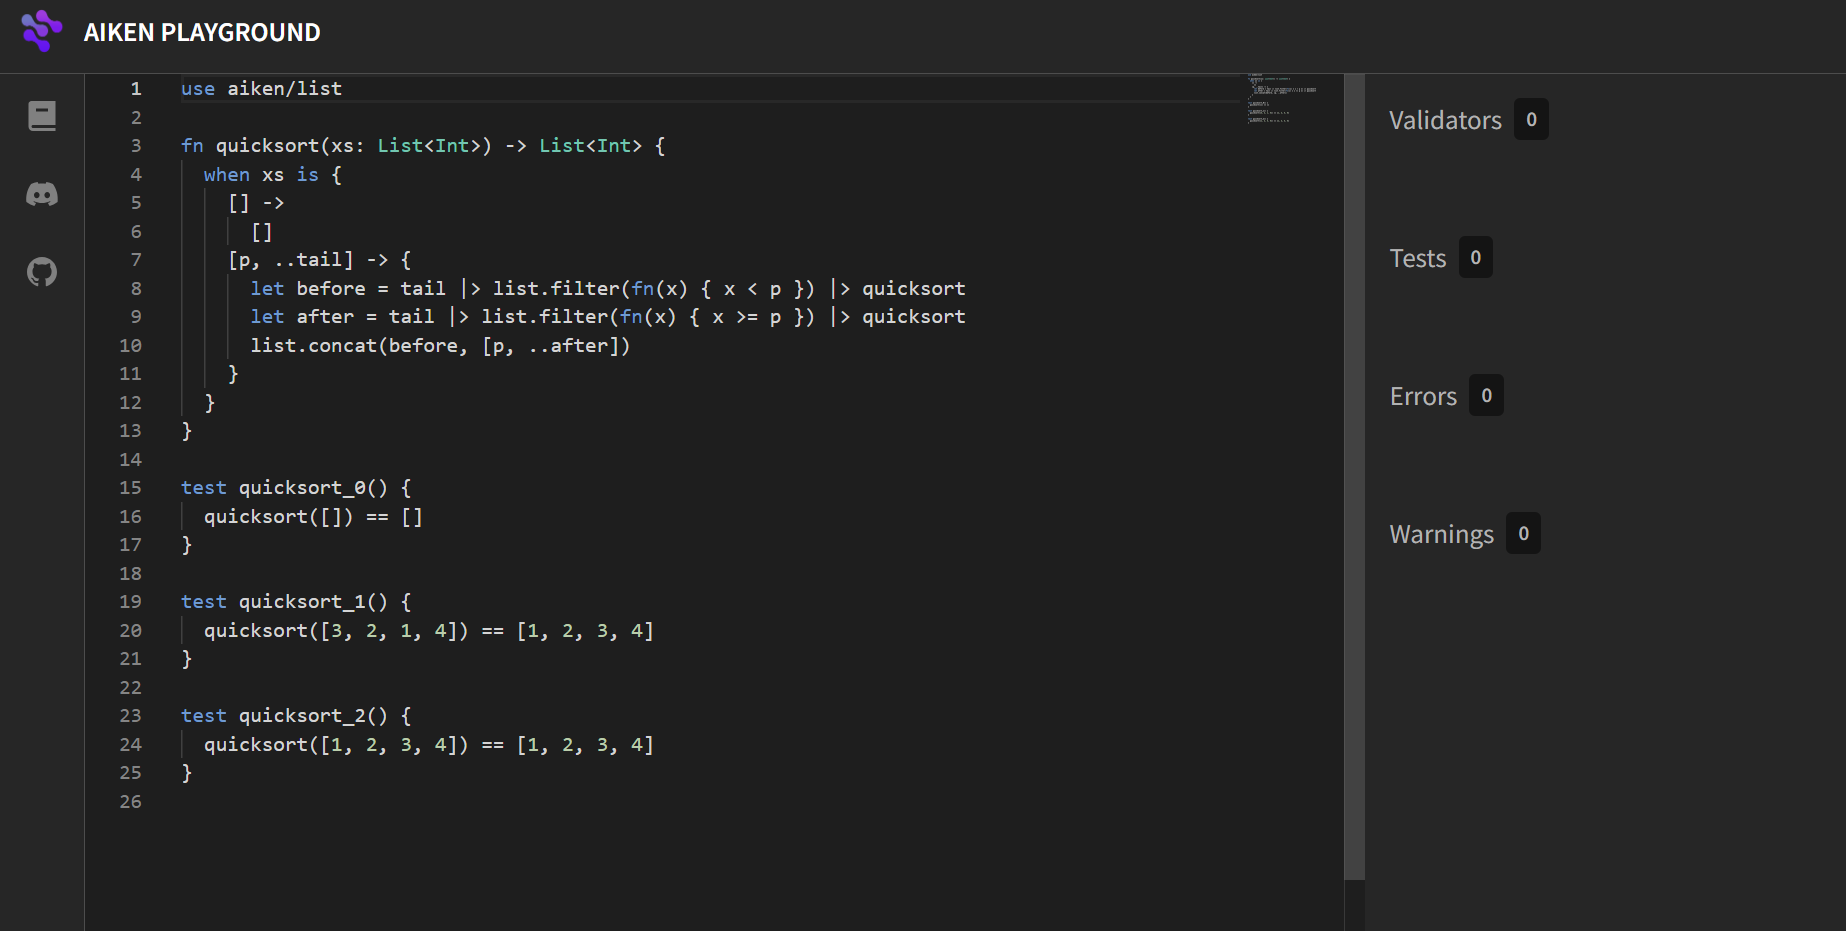
\includegraphics[scale=0.3]{aiken.png}

The Aiken Playground (\url{https://play.aiken-lang.org/}) is an online environment where developers can test and experiment with Aiken functions and smart contracts without needing to download and install the software on their local device. Similar to the Helios playground, this tool provides an easy and accessible way to get started with Aiken, allowing users to write, compile, and run Aiken code directly in the browser. It is especially useful for learning and prototyping, providing a convenient platform for exploring Aiken's features and capabilities.


\subsection{Example of a Smart Contract with Aiken}

In Aiken, we need to manually define the import libraries at the very beginning of the contract. Then, similar to Helios, we define the \texttt{Redeemer} and \texttt{Datum} types. The following smart contract will unlock the UTXO if the signer is the owner and the redeemer is the right user.

\begin{lstlisting}[language=Haskell]
use aiken/hash.{Blake2b_224, Hash}
use aiken/list
use aiken/transaction.{ScriptContext}
use aiken/transaction/credential.{VerificationKey}

type Datum {
  owner: Hash<Blake2b_224, VerificationKey>,
}

type Redeemer {
  msg: ByteArray,
}

validator {
  fn hello_world(datum: Datum, redeemer: Redeemer, context: ScriptContext) -> Bool {
    let must_say_hello =
      redeemer.msg == "Hello, World!"

    let must_be_signed =
      list.has(context.transaction.extra_signatories, datum.owner)

    must_say_hello && must_be_signed
  }
}
\end{lstlisting}


\section{OpShin Language: Concepts and Usage} \label{sec:Languages}

Opshin is an implementation of smart contracts for Cardano which are written in a strict subset of valid Python. The general philosophy of this project is to write a compiler that ensures the following:

\begin{itemize}
  \item If the program compiles, then:
  \begin{itemize}
    \item It is a valid Python program.
    \item The output running it with Python is the same as running it on-chain.
  \end{itemize}
\end{itemize}

\subsection{Why Opshin?}
\begin{itemize}
  \item \textbf{100\% valid Python:} Leverage the existing tool stack for Python, including syntax highlighting, linting, debugging, unit-testing, property-based testing, and verification.
  \item \textbf{Intuitive:} Just like Python.
  \item \textbf{Flexible:} Imperative, functional, the way you want it.
  \item \textbf{Efficient \& Secure:} Static type inference ensures strict typing and optimized code.
\end{itemize}

Opshin is a pythonic language for writing smart contracts on the Cardano blockchain. The goal of Opshin is to reduce the barrier of entry in smart contract development on Cardano. Opshin is a strict subset of Python, meaning anyone who knows Python can get up to speed with Opshin quickly.

\subsection{Setting Up the Environment}

Check out the \href{https://book.opshin.dev/}{OpShin Book} for an introduction to this tool and detailed guidance on writing smart contracts. This section outlines the basic usage of the tool.

\subsection{Installation}
Install Python 3.8, 3.9, 3.10, or 3.11. Then run:
\begin{verbatim}
python3 -m pip install opshin
\end{verbatim}

\subsection{Example of a Smart Contract}

\subsection{Example Validator - Gift Contract}
In this simple example, we'll write a gift contract that will allow a user to create a gift UTXO that can be spent by:

\begin{enumerate}
  \item The creator cancelling the gift and spending the UTXO.
  \item The recipient claiming the gift and spending the UTXO.
\end{enumerate}

\begin{lstlisting}[language=Python, caption=Gift Contract in Opshin]
# gift.py

# The Opshin prelude contains a lot of useful types and functions 
from opshin.prelude import *

# Custom Datum
@dataclass()
class GiftDatum(PlutusData):
    # The public key hash of the gift creator.
    # Used for cancelling the gift and refunding the creator (1).
    creator_pubkeyhash: bytes

    # The public key hash of the gift recipient.
    # Used by the recipient for collecting the gift (2).
    recipient_pubkeyhash: bytes

def validator(datum: GiftDatum, redeemer: None, context: ScriptContext) -> None:
    # Check that we are indeed spending a UTxO
    assert isinstance(context.purpose, Spending), "Wrong type of script invocation"

    # Confirm the creator signed the transaction in scenario (1).
    creator_is_cancelling_gift = datum.creator_pubkeyhash in context.tx_info.signatories

    # Confirm the recipient signed the transaction in scenario (2).
    recipient_is_collecting_gift = datum.recipient_pubkeyhash in context.tx_info.signatories

    assert creator_is_cancelling_gift or recipient_is_collecting_gift, "Required signature missing"
\end{lstlisting}

This might be a bit to take in, especially the logic for checking the signatures. The most important part is to see the parameters and the return type, as well as the assert statements actually controlling the validation. For more details, refer to the \href{https://book.opshin.dev/}{OpShin Book}.

\section{Plu-ts: Understanding the basics} \label{sec:Languages}

Plu-ts is a library designed for building Cardano dApps in an efficient and developer-friendly way. It is composed of two main parts:

\begin{itemize}
    \item \textbf{plu-ts/onchain:} An eDSL (embedded Domain Specific Language) that leverages TypeScript as the host language, designed to generate efficient Smart Contracts.
    \item \textbf{plu-ts/offchain:} A set of classes and functions that allow reuse of onchain types.
\end{itemize}

\subsection{Design Principles}
Plu-ts was designed with the following goals in mind, in order of importance:

\begin{itemize}
    \item \textbf{Smart Contract efficiency}
    \item \textbf{Developer experience}
    \item \textbf{Reduced script size}
    \item \textbf{Readability}
\end{itemize}

For more information, see the \href{https://book.plu-ts.dev/}{Plu-ts Book}.

\subsection{Setting Up the Environment}


\textbf{From npm:}
\begin{verbatim}
npm install @harmoniclabs/plu-ts
\end{verbatim}

\textbf{NPM:}
NPM is the package manager used by NodeJS. You can install Node and NPM from the \href{https://nodejs.org/}{NodeJS website}.

\textbf{From source:}
\begin{verbatim}
git clone https://github.com/HarmonicLabs/plu-ts
cd plu-ts
npm run build
\end{verbatim}

\textbf{The dist Folder:}
The library is then available in the \texttt{dist} folder. You can move the directory where you need it.

\subsection{Quick Start}
First, create a new directory where to build your project:
\begin{verbatim}
mkdir my-pluts-project
cd my-pluts-project
\end{verbatim}

Then initialize your Node project with npm:
\begin{verbatim}
npm init
\end{verbatim}

Install TypeScript and the TypeScript compiler \texttt{tsc} if it is not already available globally:
\begin{verbatim}
npm install --save-dev typescript
\end{verbatim}

Finally, install Plu-ts:
\begin{verbatim}
npm install @harmoniclabs/plu-ts
\end{verbatim}

\subsection{Example of a Smart Contract}

\subsection{The Contract}
In this example, we'll write a contract that expects a \texttt{MyDatum}, a \texttt{MyRedeemer}, and finally a \texttt{PScriptContext} to validate a transaction.



\begin{lstlisting}
import { Address, bool, compile, makeValidator, PaymentCredentials, pBool, pfn, Script, ScriptType, V2 } from "@harmoniclabs/plu-ts";
import MyDatum from "./MyDatum";
import MyRedeemer from "./MyRedeemer";

export const contract = pfn([
    MyDatum.type,
    MyRedeemer.type,
    V2.PScriptContext.type
],  bool)
(( datum, redeemer, ctx ) =>
    // always succeeds
    pBool( true )
);

export const untypedValidator = makeValidator( contract );
export const compiledContract = compile( untypedValidator );
export const script = new Script(
    ScriptType.PlutusV2,
    compiledContract
);

export const scriptMainnetAddr = new Address(
    "mainnet",
    new PaymentCredentials(
        "script",
        script.hash
    )
);

export const scriptTestnetAddr = new Address(
    "testnet",
    new PaymentCredentials(
        "script",
        script.hash.clone()
    )
);

export default contract;
\end{lstlisting}

This contract expects a \texttt{MyDatum}, a \texttt{MyRedeemer}, and a \texttt{PScriptContext} to validate a transaction.

\subsubsection{Custom Datum and Redeemer}
\texttt{MyDatum} and \texttt{MyRedeemer} are types defined by us in \texttt{src/MyDatum/index.ts} and \texttt{src/MyRedeemer/index.ts} respectively.

\begin{lstlisting}
import { int, pstruct } from "@harmoniclabs/plu-ts";

// modify the Datum as you prefer
const MyDatum = pstruct({
    Num: {
        number: int
    },
    NoDatum: {}
});

export default MyDatum;
\end{lstlisting}

\begin{lstlisting}
import { pstruct } from "@harmoniclabs/plu-ts";

// modify the Redeemer as you prefer
const MyRedeemer = pstruct({
    Option1: {},
    Option2: {}
});

export default MyRedeemer;
\end{lstlisting}

\subsubsection{Entry Point}
Finally, the contract is used in \texttt{src/index.ts}, which is our entry point.

\begin{lstlisting}
import { script } from "./contract";

console.log("validator compiled successfully! 🎉\n");
console.log(
    JSON.stringify(
        script.toJson(),
        undefined,
        2
    )
);
\end{lstlisting}

This index file imports the script from \texttt{src/contract.ts} and prints it out in JSON form. In this example, we see something different; instead of writing everything in the same file, we split it into several files to increase readability.

Also, note that the current contract always returns \texttt{true} as output, therefore it will always unlock the UTXO.

For more details, refer to the \href{https://book.plu-ts.dev/}{Plu-ts Book}.

The Plu-ts contract above is divided into the following key files:
\begin{itemize}
  \item \texttt{src/contract.ts} - Contains the main validator function and the script logic.
  \item \texttt{src/MyDatum/index.ts} - Defines the data structure for the Datum.
  \item \texttt{src/MyRedeemer/index.ts} - Defines the data structure for the Redeemer.
  \item \texttt{src/index.ts} - Serves as the entry point, importing and displaying the compiled script.
\end{itemize}

This organization enhances readability and separates concerns, making it easier for developers to manage and understand the contract's different components. 

In the provided example, the contract always returns \texttt{true} as the output.
This means that the contract will always validate successfully, effectively always unlocking the UTXO. While this makes the contract straightforward, it also means that the contract does not perform any meaningful validation or logic checks. 

\part{Smart Contract Runtime and Execution}
%----------------------------------------------------------------------------------------
\newpage
\chapter{Smart Contract Runtime and Execution} \label{ch:Runtime}
\section{Smart Contract Runtime and Execution} \label{sec:Runtime}


\textit{This part has been updated to be Chang compatible. The code here is already compatible with DReps, the new Aiken version, and Plutus v3.}

\subsection{Overview of Cardano's Smart Contract Execution Model}

Smart contracts on Cardano are simple constructs based on \textbf{validator scripts}. These scripts define the logic or rules to be enforced by Cardano nodes when a transaction attempts to move a UTXO locked inside the script's address.

Validator scripts can access the \textbf{transaction context} (e.g., who signed it, and which assets are sent to/from where) and the \textbf{datum} of the locked UTXO being moved, allowing the creation of complex contracts. For instance:
\begin{quote}
With smart contracts, we can add conditions to stake delegation, withdraw Cardano rewards from the protocol, or create minting policies with more dynamic conditions than regular ones.
\end{quote}

Validator scripts are executed with three main arguments:
\begin{itemize}
    \item \textbf{Datum:} Attached to the output locked by the script, often carrying state.
    \item \textbf{Redeemer:} Attached to the spending input, typically providing an input to the script. For example, a validator can apply the redeemer to the datum and verify it matches the output UTXO datum.
    \item \textbf{Context:} Contains transaction-level information, used to assert properties like “Bob signed it.”
\end{itemize}

\textbf{Transaction context properties:}
\begin{center}
\begin{tabular}{|l|p{10cm}|}
\hline
\textbf{Property} & \textbf{Description} \\
\hline
\textbf{inputs} & Outputs to be spent. \\
\textbf{reference inputs} & Inputs used for reference only, not spent. \\
\textbf{outputs} & New outputs created by the transaction. \\
\textbf{fees} & Transaction fees. \\
\textbf{minted value} & Minted or burned value. \\
\textbf{certificates} & Digest of certificates in the transaction. \\
\textbf{withdrawals} & Used to withdraw rewards from the stake pool. \\
\textbf{valid range} & Time range in which the transaction is valid. \\
\textbf{signatories} & List of transaction signatures. \\
\textbf{redeemers} & Data used as input to the script. \\
\textbf{id} & Transaction identification. \\
\hline
\end{tabular}
\end{center}

\subsection{Understanding the Transaction Context Table}

\textbf{Inputs:} These represent UTXOs being \textit{spent} in the transaction. In the UTXO model, every transaction produces outputs, which in turn become inputs for future transactions. Understanding this flow is key to interpreting inputs and outputs.

\textbf{Outputs:} These are the new UTXOs created by the transaction, ready to be used as inputs in subsequent transactions.

\textbf{Fees:} The amount of lovelace spent for transaction execution. This value is predictable and depends on the transaction size. Fees can often be optimized.

\textbf{Minted Value:} This indicates any minting or burning of tokens that occurs in the transaction.

\textbf{Certificates:} Information about stake operations. For example:
\begin{itemize}
    \item Registering a stake key.
    \item Delegating to a DRep.
\end{itemize}

\textbf{Withdrawals:} Rewards withdrawn from stake keys. For example, if you use a wallet like Lace, which allows delegation to multiple pools, you may see multiple withdrawals in one transaction.

\textbf{Valid Range:} A time frame during which the transaction is valid. This is useful for ensuring a transaction only executes within specific boundaries.

\textbf{Signatories:} A list of hashes representing who signed the transaction. This is essential for multi-signature transactions.

\textbf{Redeemers:} A list of redeemers used by the contracts executed in the transaction.

\textbf{ID:} The transaction hash, uniquely identifying the transaction.

During runtime, each validator checks its \textit{datum}, \textit{redeemer}, and the \textit{context} (or local transaction state).

\textbf{Important exercise:} 
Imagine a transaction that:
\begin{itemize}
    \item Spends \textbf{three different UTXOs} from the same contract.
    \item Withdraws staking rewards from a stake key contract.
    \item Mints \textbf{two different tokens} under separate contract policies.
\end{itemize}

\textit{Questions:}
\begin{enumerate}
    \item How many unique contracts are executed?
    \item How many datums are present?
    \item How many redeemers?
\end{enumerate}

\textbf{Answer:} After a blank page—\textit{Take your time; don’t rush!}
\newpage
\thispagestyle{empty}
\textbf{Real answer:}

\begin{enumerate}
    \item 4
    \item 3
    \item 6
\end{enumerate}

Did you get them? Let's try to understand why.
Spending inputs from a contract, even if it's coming from the same contract is treated like a unique execution.
Therefore for each input coming from contract A, we will have it's own Datum and it's own redeemer. 

Withdraw and minting contract do not have datums, they have redeemers.
You can mint or withdraw from the same contract only once, therefore the logic behind these contracts must be more flexible to allow different logic inside the same execution.

It will be easier to understand at the end of this chapter, you need to take home this:

\begin{quote}
    SPEND contracts are executed once for each input, while minting and withdrawals contracts are executed once for each transaction
\end{quote}



\section{Transaction Verification and Script Validation}


To understand transaction validation on Cardano, it is crucial to recognize that even if a script validates a transaction, the transaction might still fail due to the network's robust two-phase validation mechanism. This section explores this process and the role of collateral in ensuring successful smart contract execution.

\subsubsection{Two-Phase Validation Mechanism}

Cardano employs a two-phase validation scheme to minimize uncompensated work for nodes, ensuring efficiency and security:

\begin{itemize}
    \item \textbf{Phase 1: Structural Validation}
    \begin{itemize}
        \item Checks if the transaction is correctly constructed.
        \item Ensures that the transaction can pay its processing fee.
        \item If Phase 1 fails, the transaction is immediately discarded without running any scripts.
    \end{itemize}
    \item \textbf{Phase 2: Script Execution}
    \begin{itemize}
        \item Executes the scripts included in the transaction.
        \item If a script fails, the transaction fails, and collateral is used to compensate nodes.
    \end{itemize}
\end{itemize}

\subsubsection{The Role of Collateral}
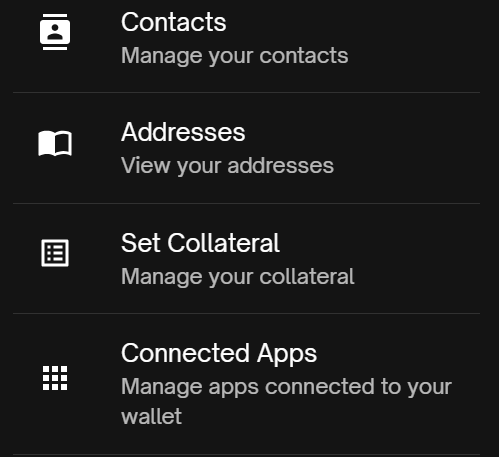
\includegraphics{collateral.png}

Collateral ensures that nodes are compensated for their work if Phase 2 validation fails. It acts as a monetary guarantee, encouraging careful design and testing of smart contracts. Key details about collateral:

\begin{itemize}
    \item \textbf{Collateral Inputs:} The collateral amount is determined by the total balance of UTXOs marked as collateral inputs.
    \item \textbf{Safety for Honest Users:} Collateral is not collected if a transaction succeeds or is invalid at Phase 1.
    \item \textbf{Deterministic Costs:} Cardano's deterministic design allows users to calculate execution costs and collateral requirements in advance, unlike Ethereum where gas costs can vary based on network activity.
    \item \textbf{Vasil Upgrade Improvement:} Developers can specify a change address for script collateral, ensuring only the required amount is taken if a script fails, with the remainder returned to the specified address.
\end{itemize}

\subsubsection{Importance of Collateral}

Without collateral, malicious actors could exploit the network by flooding it with invalid transactions at little cost. By requiring collateral, Cardano ensures:

\begin{itemize}
    \item Transactions calling non-native (Phase 2) smart contracts include sufficient collateral to cover potential failure costs.
    \item Denial of Service (DoS) attacks become prohibitively expensive.
    \item Honest users never lose their collateral as long as transactions are valid and successful.
\end{itemize}

\subsubsection{Technical Details}

Phase 2 scripts on Cardano can perform arbitrary computations and require a budget of execution units (ExUnits) to quantify resource usage. This budget is included in the transaction fee calculation. Collateral provides additional safeguards:

\begin{itemize}
    \item \textbf{Multi-Signature Scripts:} Introduced in the Shelley era, Phase 1 scripts follow deterministic ledger rules, enabling straightforward cost assessment.
    \item \textbf{ExUnit Budgeting:} Phase 2 scripts require a resource budget for metrics like memory usage and execution steps, ensuring fair cost allocation.
\end{itemize}

The Cardano testnet provides a safe environment with free test ADA, enabling developers to rigorously test smart contracts before deploying them on the mainnet. This ensures that transactions and scripts function correctly under real-world conditions.


\section{Debugging and Troubleshooting Smart Contracts}

Debugging smart contracts can be challenging, but interacting directly with the blockchain is not always necessary. Thanks to tools like Aiken and Gastronomy, developers can efficiently test and debug their smart contracts in a controlled environment.

\subsubsection{Debugging with Aiken}

Aiken offers first-class support for unit tests and property-based tests, allowing developers to write and execute tests directly in Aiken without deploying to the blockchain. The toolkit (`aiken check`) parses tests, runs them, and displays detailed reports.

\paragraph{Unit Tests}

Unit tests in Aiken are written using the `test` keyword. A test is a named function that takes no arguments and returns a boolean. It is valid (i.e., it passes) if it returns `True`.

\begin{verbatim}
test foo() {
  1 + 1 == 2
}
\end{verbatim}

Unit tests can call functions and use constants, and they execute on the same virtual machine used for on-chain contracts. This ensures that tests mirror the production environment.

\paragraph{Example Unit Tests}

\begin{verbatim}
lib/example.ak
fn add_one(n: Int) -> Int {
  n + 1
}
 
test add_one_1() {
  add_one(0) == 1
}
 
test add_one_2() {
  add_one(-42) == -41
}
\end{verbatim}

Running `aiken check` generates a report grouping tests by module and displaying the memory and CPU execution units needed for each test. This report can also be used as a benchmark to compare execution costs of different approaches.

Tests in Aiken can be as complex as necessary, without the execution limits imposed on on-chain scripts.

\paragraph{Trace and Debugging}

Aiken supports debugging via CBOR diagnostic traces. Developers can use `trace` to print diagnostic data (e.g., integers or byte arrays) in the event of a contract failure. If the contract succeeds, no output is shown.

\begin{verbatim}
// An Int becomes a CBOR int
trace cbor.diagnostic(42)
 
// A ByteArray becomes a CBOR bytestring
trace cbor.diagnostic("foo")
\end{verbatim}

This feature provides valuable insights during debugging by simulating breakpoints.

\subsubsection{Advanced Debugging with Gastronomy}

\includegraphics[scale=0.3]{gastronomy.png}
Gastronomy, developed by Sundae Labs, is a powerful UPLC debugger designed to aid in diagnosing failed scripts based on error codes. It allows developers to step through script execution with ease.

\paragraph{Features}

\begin{itemize}
    \item Stores the state of the machine at every execution step.
    \item Allows stepping forward and backward to analyze script behavior.
    \item Provides a user-friendly interface for debugging.
\end{itemize}

\paragraph{Quick Start}

\textbf{CLI Tool:}
\begin{verbatim}
gastronomy-cli run test_data/fibonacci.uplc 03
N - Advance to the next step
P - Rewind to the previous step
Q - Quit
\end{verbatim}

\textbf{GUI Tool:}
Simply run `gastronomy` to launch the graphical interface.

\paragraph{Configuration}

Gastronomy can be configured using environment variables or a `.gastronomyrc.toml` file in the home directory. Example configuration:

\begin{verbatim}
    Setting          Environment Variable     Description
    blockfrost.key   BLOCKFROST_KEY           The API key to use when querying Blockfrost.
\end{verbatim}




By leveraging Aiken and Gastronomy, developers can thoroughly test and debug their smart contracts, ensuring reliability and efficiency before deployment.


\section{Tx Optimization Techniques for Efficient Execution}

In recent years, several effective techniques have been discovered to optimize smart contracts on Cardano. Many of these can be found in the repository at \href{https://github.com/Anastasia-Labs/aiken-design-patterns}{Aiken Design Patterns}. Here, we will discuss two game-changing techniques: the "Withdraw 0 Trick" and "Parametric Scripts."

\subsubsection{Withdraw 0 Trick}

The "Withdraw 0 Trick" is particularly useful for validators that need to handle multiple inputs efficiently. By splitting logic into two distinct parts—a minimal spending logic and an arbitrary withdrawal logic—scripts can be made significantly more efficient. 

\paragraph{How It Works}

Withdraw scripts are executed only once per transaction, whereas spend validators are executed once for every input originating from the same smart contract. For example, if purchasing multiple NFTs from a marketplace, the transaction's execution logic grows proportionally to the number of NFTs.

Using the "Withdraw 0 Trick," this logic is split:
\begin{itemize}
    \item The spend validator checks that a "withdraw 0" operation is executed.
    \item The withdrawal logic is handled independently in the "withdraw 0" contract, decoupling it from the number of NFTs.
\end{itemize}

This approach reduces complexity, ensures scalability, and maintains elegance in design.

\paragraph{Implementation Details}

The module offers two key functions for spending endpoints:
\begin{itemize}
    \item \textbf{spend} \textendash{} Traverses both the withdrawals and redeemers fields, validating against both the redeemer and the withdrawal quantity.
    \item \textbf{spend\_minimal} \textendash{} Traverses only the withdrawals, ideal when no validation is needed on the staking script's redeemer or withdrawal quantity.
\end{itemize}

Additionally, the \textbf{withdraw} function unwraps the staking credential and provides the underlying hash, facilitating minimal execution logic.

\subsubsection{Parametric Scripts}

Parametric scripts are another crucial optimization technique, significantly enhancing execution efficiency by predefining key parameters within the script itself.

\paragraph{Why Use Parametric Scripts?}

Certain contracts require specific parameters, such as a spend contract that must identify an NFT with a matching policy script hash. Without predefined parameters, the contract would consume excessive CPU resources to compute its own script hash. By using parametric scripts, the contract already "knows" the required values, saving computation time and resources.

\paragraph{Practical Example}

Consider a minting script that restricts token destinations to instances of a specific spending script parameterized by user wallets. Each wallet results in a different script address, making verification challenging. Using parametric scripts, the minting script can:
\begin{itemize}
    \item Validate instances as the result of applying specific parameters to a parameterized script.
    \item Ensure robust asset flow control.
\end{itemize}

\paragraph{On-Chain Validation Requirements}

To validate parameterized scripts on-chain, the following restrictions apply:
\begin{itemize}
    \item Script parameters must have constant lengths (achieved via hashing).
    \item Redeemers must supply resolved values of parameters for each transaction.
    \item Dependent scripts must include CBOR bytes of instances before and after parameter application.
    \item Logic wrapping ensures a single occurrence of each parameter.
\end{itemize}

\paragraph{Implementation Steps}

Define parameterized scripts and generate instances with dummy data to obtain required prefix and postfix values. Use these values in your target script. For detailed examples, refer to \href{https://github.com/Anastasia-Labs/aiken-design-patterns}{validators/apply-params-example.ak}.

These optimization techniques provide a solid foundation for efficient, scalable smart contract execution on Cardano.


\part{Smart Contract Runtime and Execution}
%----------------------------------------------------------------------------------------
\newpage
\chapter{Getting Started with Cardano Smart Contract Development} \label{ch:Getting started}
\section{Key Concepts and Terminology}

In this chapter, we will get hands-on experience by writing a smart contract in Aiken and the corresponding off-chain code, typically implemented in the frontend using Mesh. Finally, we will submit a transaction and interact with it.

At the end of the chapter, you will also find exercises to test your understanding and skills.

\subsection{Key Concepts}

Here is a list of key concepts and terminology that will help you:

\begin{itemize}
    \item \textbf{Collateral}: A specific UTxO required to interact with smart contracts. It ensures that nodes are compensated in case the contract validation fails.
    \item \textbf{Script Hash}: A unique hash that identifies the smart contract, allowing transactions to reference it securely.
    \item \textbf{Locked UTxO}: A transaction output that holds funds, NFTs, or tokens locked within a contract. These can only be spent if the contract validation logic passes.
    \item \textbf{CIP69 Contract}: A contract where the datum is optional. It behaves like a user, allowing it to receive funds. However, every UTxO associated with this contract must execute the validation logic to be spendable.
    \item \textbf{Multipurpose Script}: A versatile script that can perform multiple functions, such as locking funds, minting NFTs, and more.
\end{itemize}


\section{Writing Your First Smart Contract}

Let's write and execute a smart contract on Cardano in 10 minutes. Yes, you read that right.

You can find code supporting this tutorial on Aiken's main repository.

\subsection{Covered in this tutorial}
\begin{itemize}
    \item Writing a basic Aiken validator;
    \item Writing \& running tests with Aiken;
    \item Troubleshooting smart contracts.
\end{itemize}

When encountering an unfamiliar syntax or concept, do not hesitate to refer to the language-tour for details and extra examples.

\subsection{Pre-requisites}
We'll use Aiken to write the script, so make sure the command-line tool is installed already. Otherwise, refer to the installation instructions.

\subsection{Scaffolding}
First, let's create a new Aiken project:

\begin{verbatim}
aiken new aiken-lang/hello-world
cd hello-world
\end{verbatim}

This command scaffolds an Aiken project. In particular, it creates a \texttt{lib} and \texttt{validators} folder in which you can put Aiken source files.

\begin{verbatim}
./hello-world
│
├── README.md
├── aiken.toml
├── lib
└── validators
\end{verbatim}

\subsection{Using the standard library}
We'll use the standard library for writing our validator. Fortunately, \texttt{aiken new} did automatically add the standard library to our \texttt{aiken.toml} for us. It should look roughly like that:

\begin{verbatim}
aiken.toml
name = "aiken-lang/hello-world"
version = "0.0.0"
license  = "Apache-2.0"
description = "Aiken contracts for project 'aiken-lang/hello-world'"
 
[repository]
user = 'aiken-lang'
project = 'hello-world'
platform = 'github'
 
[[dependencies]]
name = "aiken-lang/stdlib"
version = "v2"
source = "github"
\end{verbatim}

Now, running \texttt{aiken check}, we should see dependencies being downloaded. That shouldn't take long.

\begin{verbatim}
❯ aiken check
    Compiling aiken-lang/hello-world 1.0.0 (examples/hello-world/)
    Resolving aiken-lang/hello-world
      Fetched 1 package in 0.01s from cache
    Compiling aiken-lang/stdlib v2 (/Users/aiken/Documents/aiken-lang/hello-world/build/packages/aiken-lang-stdlib)
      Summary 0 errors, 0 warnings
\end{verbatim}

\subsection{Our First Validator}
Let's write our first validator as \texttt{validators/hello\_world.ak}:

\begin{verbatim}
validators/hello_world.ak
use aiken/collection/list
use aiken/crypto.{VerificationKeyHash}
use cardano/transaction.{OutputReference, Transaction}
 
pub type Datum {
  owner: VerificationKeyHash,
}
 
pub type Redeemer {
  msg: ByteArray,
}
 
validator hello_world {
  spend(
    datum: Option<Datum>,
    redeemer: Redeemer,
    _own_ref: OutputReference,
    self: Transaction,
  ) {
    expect Some(Datum { owner }) = datum
    let must_say_hello = redeemer.msg == "Hello, World!"
    let must_be_signed = list.has(self.extra_signatories, owner)
    must_say_hello && must_be_signed
  }
}
\end{verbatim}

Our first validator is rudimentary, yet there's already a lot to say about it.

It looks for a verification key hash (\texttt{owner}) in the datum and a message (\texttt{msg}) in the redeemer. Remember that, in the eUTxO model, the datum is set when locking funds in the contract and can be seen as configuration. Here, we'll indicate the owner of the contract and require a signature from them to unlock funds—very much like it already works on a typical non-script address.

Moreover, because there's no "Hello, World!" without a proper "Hello, World!", our little contract also demands this very message, as a UTF-8-encoded byte array, to be passed as redeemer (i.e. when spending from the contract).

It's now time to build our first contract!

\begin{verbatim}
aiken build
\end{verbatim}

This command generates a CIP-0057 Plutus blueprint as \texttt{plutus.json} at the root of your project. This blueprint describes your on-chain contract and its binary interface. In particular, it contains the generated on-chain code that will be executed by the ledger and a hash of your validator(s) that can be used to construct addresses.

This format is framework-agnostic and is meant to facilitate interoperability between tools. The blueprint is fully integrated into Aiken, which can automatically generate it based on your type definitions and comments.

\subsection{Let's see the validator in action!}

\begin{itemize}
    \item Interact with a validator on the Preview network;
    \item Using Mesh through Blockfrost;
    \item Getting test funds from the Cardano Faucet;
    \item Using web explorers such as CardanoScan.
\end{itemize}

\subsection{Pre-requisites}
We assume that you have followed the "Hello, World!"'s First steps and thus, have Aiken installed and ready-to-use. We will also use Mesh, so make sure you have your dev environment ready for some JavaScript!.

You can install Mesh and set up the project as follows:

\begin{verbatim}
npm init -y
npm install @meshsdk/core tsx
\end{verbatim}

\subsection{Getting Funds}
For this tutorial, we will use the validator we built in First steps. Yet, before moving on, we'll need some funds, and a public/private key pair to hold them. We can generate a private key and an address using MeshWallet.

\begin{verbatim}
generate-credentials.ts
import { MeshWallet } from '@meshsdk/core';
import fs from 'node:fs';
 
const secret_key = MeshWallet.brew(true) as string;
 
fs.writeFileSync('me.sk', secret_key);
 
const wallet = new MeshWallet({
  networkId: 0,
  key: {
    type: 'root',
    bech32: secret_key,
  },
});
 
fs.writeFileSync('me.addr', wallet.getUnusedAddresses()[0]);
\end{verbatim}

You can run the instructions above via:

\begin{verbatim}
npx tsx generate-credentials.ts
\end{verbatim}

Now, we can head to the Cardano faucet to get some funds on the preview network to our newly created address (inside \texttt{me.addr}).

Make sure to select "Preview Testnet" as the network.

Using CardanoScan, we can watch for the faucet sending some ADA our way. This should be pretty fast (a couple of seconds).

\section{Deploying and Interacting with Smart Contracts}
No need to deploy like in ethereum, as soon as we send a transaction in the contract we are ready to go.

Now that we have some funds, we can lock them in our newly created contract. We'll use Blockfrost Provider to construct and submit our transaction through Blockfrost.

This is only one example of a possible setup using tools we love. For more tools, make sure to check out the Cardano Developer Portal!

\subsection{Setup}
First, we set up Mesh with Blockfrost as a provider. This will allow us to let Mesh handle transaction building for us, which includes managing changes. It also gives us a direct way to submit the transaction later on.

\begin{verbatim}
common.ts
import fs from "node:fs";
import {
  BlockfrostProvider,
  MeshTxBuilder,
  MeshWallet,
  serializePlutusScript,
  UTxO,
} from "@meshsdk/core";
import { applyParamsToScript } from "@meshsdk/core-csl";
 
const blockchainProvider = new BlockfrostProvider(process.env.BLOCKFROST_PROJECT_ID);
 
// wallet for signing transactions
export const wallet = new MeshWallet({
  networkId: 0,
  fetcher: blockchainProvider,
  submitter: blockchainProvider,
  key: {
    type: "root",
    bech32: fs.readFileSync("me.sk").toString(),
  },
});
\end{verbatim}

Note that the highlighted line above looks for an environment variable named \texttt{BLOCKFROST\_PROJECT\_ID} which its value must be set to your Blockfrost project id. You can define a new environment variable in your terminal by running (in the same session you're also executing the script!):

\begin{verbatim}
export BLOCKFROST_PROJECT_ID=preview...
\end{verbatim}

Replace \texttt{preview...} with your actual project id.

\subsection{Locking Funds into the Contract}
Now that we can read our validator, we can make our first transaction to lock funds into the contract. The datum must match the representation expected by the validator (and as specified in the blueprint), so this is a constructor with a single field that is a byte array.

\begin{verbatim}
lock.ts
import { Asset, deserializeAddress, mConStr0 } from "@meshsdk/core";
import { getScript, getTxBuilder, wallet } from "./common";
 
async function main() {
  // these are the assets we want to lock into the contract
  const lockAmount = 10_000_000;
 
  // get a valid address for the contract
  const validatorAddr = deserializeAddress(
    "addr_test1qxygsw9r9rt5q0jx8m6lmcjlsrn2ck7c7tpekl9wzyj8nvc70wwdlcs78s7ntljtm6xqfvwzttttts33dtjpytldc7cs7dpjl7jqxyr9qyz3e"
  );
 
  // lock the funds!
  const { tx, requiredSigners } = await getTxBuilder().build({
    assets: [new Asset("lovelace", lockAmount)],
    recipients: [
      {
        address: validatorAddr,
        datum: { owner: wallet.getUnusedAddresses()[0] },
      },
    ],
  });
  await wallet.signAndSubmit(tx, requiredSigners);
}
 
main();
\end{verbatim}


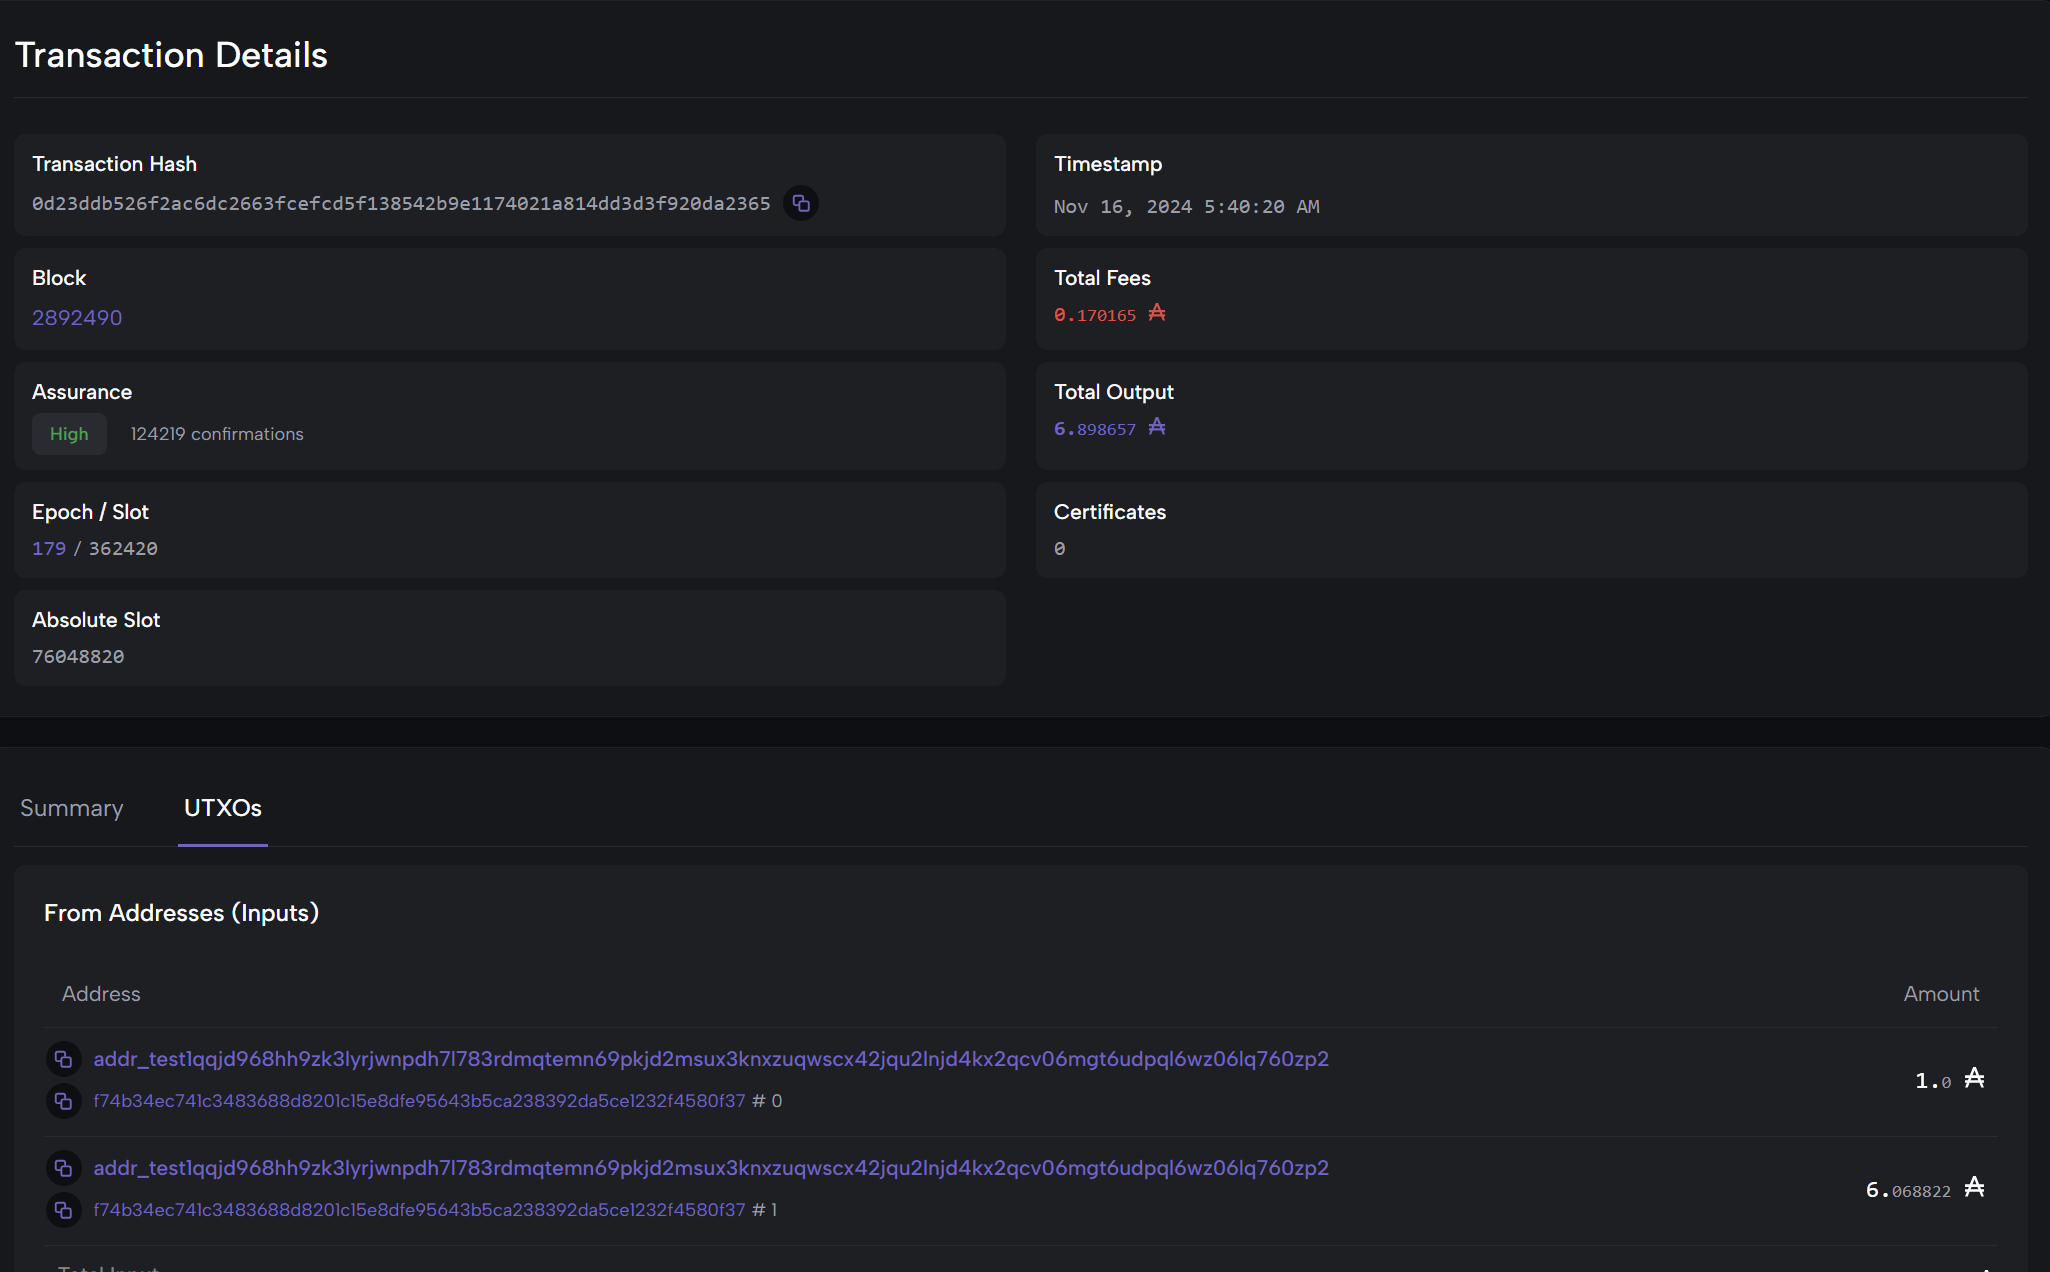
\includegraphics[scale=0.3]{lock.png}


Once again, you may check the transaction on CardanoScan.

\subsection{Spending from the Contract}
With our funds now locked in the contract, we can now spend them. First, we'll need a transaction that spends the funds, passing in the correct redeemer with the value \texttt{Hello, World!}.

\begin{verbatim}
spend.ts
import { getTxBuilder, wallet } from "./common";
 
async function main() {
  const tx = await getTxBuilder().build({
    assets: [{ asset: "lovelace", amount: 10_000_000 }],
    recipients: [
      {
        address: wallet.getUnusedAddresses()[0],
        redeemer: { msg: "Hello, World!" },
      },
    ],
  });
  await wallet.signAndSubmit(tx);
}
 
main();
\end{verbatim}
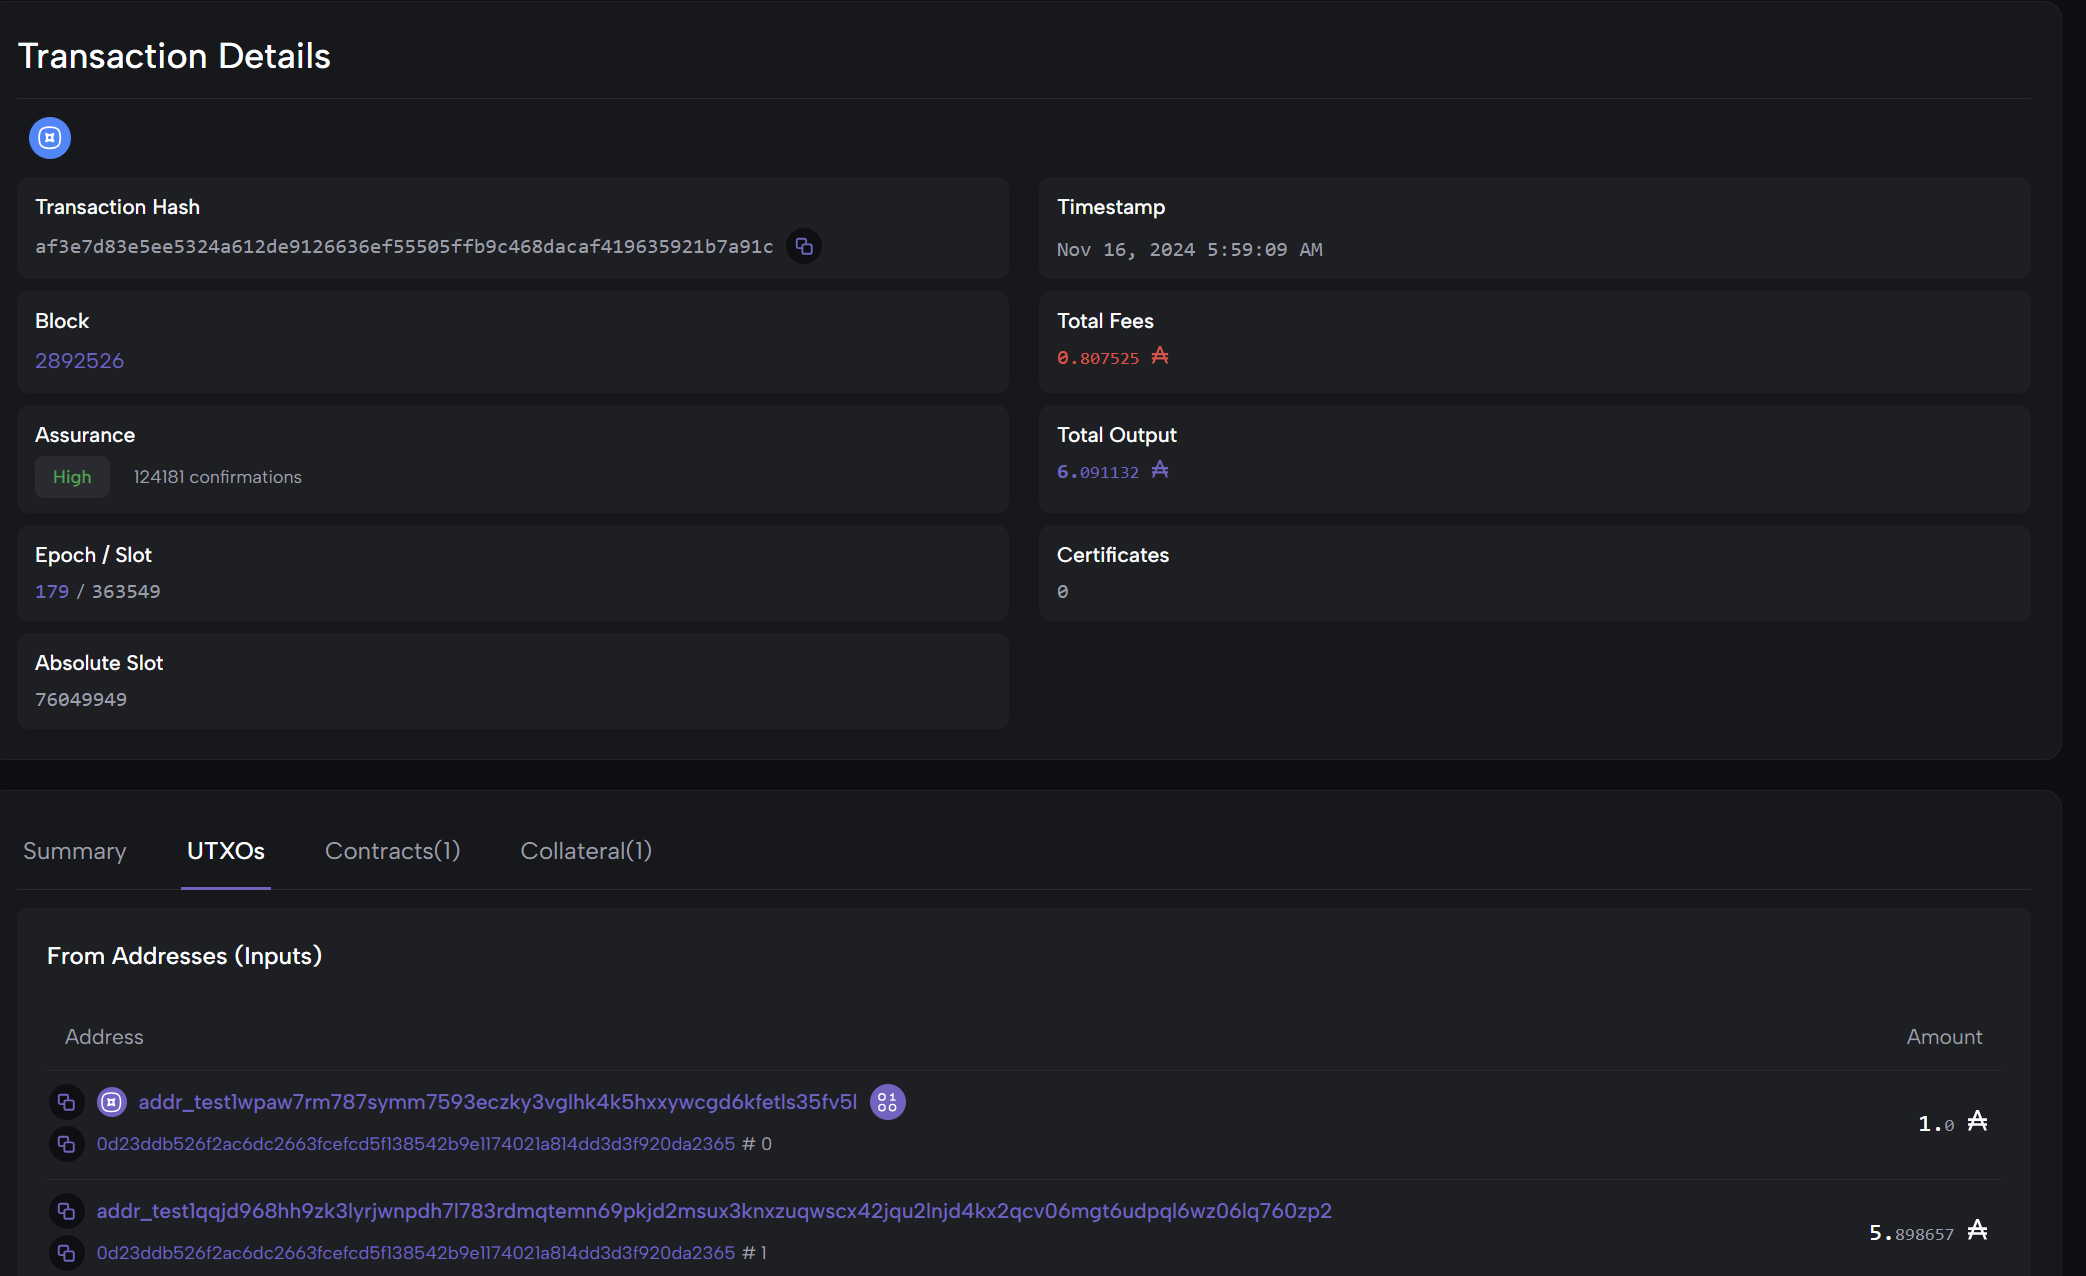
\includegraphics[scale=0.3]{unlock.png}



Once the transaction is complete, go ahead and look for it on CardanoScan again to confirm the transaction has been processed.

You can look for it using the transaction hash: \textit{af3e7d83e5ee5324a612de9126636ef55505ffb9c468dacaf419635921b7a91c}


\section{Best Practices for Secure and Robust Smart Contract}

Auditing should be mandatory before any contract goes live. While open-source code is beneficial for transparency and trust, it is not sufficient on its own. Audits help identify potential vulnerabilities and ensure that the contract behaves as expected under various conditions. 

A well-conducted audit verifies that the code meets security standards and mitigates risks, including potential exploits or misuse. Moreover, it's important to have a robust testing framework in place to ensure the contract functions correctly in both expected and edge cases.

Following these best practices ensures the safety of assets and enhances the reliability of smart contracts in decentralized applications.

Here is a list of checks that you should perform on your contract before going live:

\begin{itemize}
    \item \textbf{Dust attack:} The contract may be used by an attacker who adds additional tokens, making the UTXO locked forever.
    \item \textbf{Double spending:} Ensure that the contract logic is enforced so that it is only executed for one input at a time, preventing multiple inputs from being withdrawn from the contract.
    \item \textbf{Stake key:} Verify that funds are sent to the correct contract under the right stake key. This ensures that the true owner receives staking rewards.
    \item \textbf{Mint-burn:} Confirm that the mint or burn functions are validating the correct policy, and not just using a random asset name.
\end{itemize}

\section{Exercises to test your smart contract skills}
\begin{remark}
    EXERCISE 3: Make all tutorials available in the following links:
    \begin{itemize}
        \item \url{https://aiken-lang.org/example--vesting}
        \item \url{https://aiken-lang.org/example--gift-card}
    \end{itemize}
\end{remark}

\begin{remark}
    EXERCISE 4: Create a minting policy that allows the following:
    \begin{itemize}
        \item Mint the token \texttt{always} to everyone, at any time.
        \item Mint the token \texttt{onetime} only to the project owner, and only once forever.
        \item Mint the token \texttt{fenix} only if both \texttt{always} and \texttt{onetime} have been burned.
        \item Any other token name is forbidden.
    \end{itemize}
\end{remark}

\begin{remark}
    EXERCISE 5: Create a smart wallet account where users can receive payments. The datum is optional, as it can function like a regular wallet. The rules are as follows:
    \begin{itemize}
        \item If the datum is empty, the owner can spend the tokens.
        \item If the datum is not empty, it indicates the time when the user can withdraw it, as a POSIX timestamp.
        \item The owner can be a user, a smart contract, or a multisig, allowing multisignatures and smart contracts to use it as well.
    \end{itemize}
\end{remark}

\begin{remark}
    EXERCISE 6: Implement a contract where a user can lock 1 NFT and generate an amount of N tokens as a result. The conditions are as follows:
    \begin{itemize}
        \item The only way to unlock the NFT is to burn a number M of tokens in the transaction.
        \item The unit of the NFT, the number N of tokens generated, and the number M of tokens to burn are parameters of the contract.
    \end{itemize}
\end{remark}




\newpage
\part{EXERCISE solutions}
\chapter{Solutions}
\section{Solutions}

\subsection{Exercise 1}
\textit{You can find the solution file for easy copy and paste:} \href{https://github.com/elRaulito/eUTxO-Fundamentals-Building-Cardano-Smart-Contracts/blob/main/eBook/sections/solutions/index.html}{Solution 1 File (formatted code)}


% Define HTML language style for listings
\lstdefinelanguage{HTML}{
    sensitive=true,
    keywords={},
    otherkeywords={<, >, /, =},
    morecomment=[s]{<!--}{-->},
    morestring=[b]",
    morestring=[b]',
}

% Set listing style
\lstset{
    basicstyle=\ttfamily\small,
    commentstyle=\color{gray},
    stringstyle=\color{blue},
    keywordstyle=\color{black},
    showstringspaces=false,
    tabsize=4,
    language=HTML,
    breaklines=true,
    frame=single,
    captionpos=b
}


\lstinputlisting[]{sections/solutions/index.html}

\subsection{Exercise 2}
\textit{You can find the solution file for easy copy and paste:} \href{https://github.com/elRaulito/eUTxO-Fundamentals-Building-Cardano-Smart-Contracts/blob/main/eBook/sections/solutions/get_addresses.py}{Solution 2 File (formatted code)}

% Define Python language style for listings
\lstdefinelanguage{Python}{
  keywords={import, def, while, True, if, else, break, print, with, as, not, None},
  keywordstyle=\color{blue}\bfseries,
  ndkeywords={class, return, try, except, finally, raise},
  ndkeywordstyle=\color{orange}\bfseries,
  identifierstyle=\color{black},
  sensitive=false,
  comment=[l]{\#},
  morecomment=[s]{/*}{*/},
  commentstyle=\color{gray}\ttfamily,
  stringstyle=\color{red}\ttfamily,
  morestring=[b]',
  morestring=[b]"
}

% Set listing style
\lstset{
  basicstyle=\ttfamily\small,
  commentstyle=\color{gray},
  stringstyle=\color{green},
  keywordstyle=\color{blue},
  showstringspaces=false,
  tabsize=4,
  language=Python,
  breaklines=true,
  frame=single,
  captionpos=b
}


\lstinputlisting[]{sections/solutions/get_addresses.py}


\subsection{Exercise 3}
\textit{You can find the solution file for easy copy and paste:} \href{https://github.com/elRaulito/eUTxO-Fundamentals-Building-Cardano-Smart-Contracts/blob/main/eBook/sections/solutions/nft.ak}{Solution 3 File (formatted code)}
% Define Aiken language style for listings
\lstdefinelanguage{Aiken} {
    keywords={
        use, pub, type, validator, fn, let, if, else, when, trace, expect, and, or, fail, True, False,
        Mint, Burn, Action, Option, List, Dict, Pair, ByteArray, Int, Pairs, Input, Output, Transaction, Script, NoDatum
    },
    keywordstyle=\color{blue}\bfseries,
    ndkeywords={
        from_asset, from_asset_list, mock_policy_id, mock_pub_key_hash, mock_utxo_ref, assets, dict, list, to_string, to_bytearray
    },
    ndkeywordstyle=\color{orange}\bfseries,
    identifierstyle=\color{black},
    sensitive=false,
    comment=[l]{\#},
    morecomment=[s]{/*}{*/},
    commentstyle=\color{gray}\ttfamily,
    stringstyle=\color{red}\ttfamily,
    morestring=[b]',
    morestring=[b]"
}

% Set listing style for Aiken code
\lstset{
    basicstyle=\ttfamily\small,
    commentstyle=\color{gray},
    stringstyle=\color{red},
    keywordstyle=\color{blue},
    showstringspaces=false,
    tabsize=4,
    language=Aiken,
    breaklines=true,
    frame=single,
    captionpos=b
}



\lstinputlisting[]{sections/solutions/nft.ak}

\subsection{Exercise 4}
\textit{You can find the solution file for easy copy and paste:} \href{https://github.com/elRaulito/eUTxO-Fundamentals-Building-Cardano-Smart-Contracts/blob/main/eBook/sections/solutions/cip69.ak}{Solution 4 File (formatted code)}
% Define Aiken language style for listings
\lstdefinelanguage{Aiken} {
    keywords={
        use, pub, type, validator, fn, let, if, else, when, trace, expect, and, or, fail, True, False,
        Mint, Burn, Action, Option, List, Dict, Pair, ByteArray, Int, Pairs, Input, Output, Transaction, Script, NoDatum
    },
    keywordstyle=\color{blue}\bfseries,
    ndkeywords={
        from_asset, from_asset_list, mock_policy_id, mock_pub_key_hash, mock_utxo_ref, assets, dict, list, to_string, to_bytearray
    },
    ndkeywordstyle=\color{orange}\bfseries,
    identifierstyle=\color{black},
    sensitive=false,
    comment=[l]{\#},
    morecomment=[s]{/*}{*/},
    commentstyle=\color{gray}\ttfamily,
    stringstyle=\color{red}\ttfamily,
    morestring=[b]',
    morestring=[b]"
}

% Set listing style for Aiken code
\lstset{
    basicstyle=\ttfamily\small,
    commentstyle=\color{gray},
    stringstyle=\color{red},
    keywordstyle=\color{blue},
    showstringspaces=false,
    tabsize=4,
    language=Aiken,
    breaklines=true,
    frame=single,
    captionpos=b
}



\lstinputlisting[]{sections/solutions/cip69.ak}

\subsection{Exercise 5}
\textit{You can find the solution file for easy copy and paste:} \href{https://github.com/elRaulito/eUTxO-Fundamentals-Building-Cardano-Smart-Contracts/blob/main/eBook/sections/solutions/fraction.ak}{Solution 5 File (formatted code)}
% Define Aiken language style for listings
\lstdefinelanguage{Aiken} {
    keywords={
        use, pub, type, validator, fn, let, if, else, when, trace, expect, and, or, fail, True, False,
        Mint, Burn, Action, Option, List, Dict, Pair, ByteArray, Int, Pairs, Input, Output, Transaction, Script, NoDatum
    },
    keywordstyle=\color{blue}\bfseries,
    ndkeywords={
        from_asset, from_asset_list, mock_policy_id, mock_pub_key_hash, mock_utxo_ref, assets, dict, list, to_string, to_bytearray
    },
    ndkeywordstyle=\color{orange}\bfseries,
    identifierstyle=\color{black},
    sensitive=false,
    comment=[l]{\#},
    morecomment=[s]{/*}{*/},
    commentstyle=\color{gray}\ttfamily,
    stringstyle=\color{red}\ttfamily,
    morestring=[b]',
    morestring=[b]"
}

% Set listing style for Aiken code
\lstset{
    basicstyle=\ttfamily\small,
    commentstyle=\color{gray},
    stringstyle=\color{red},
    keywordstyle=\color{blue},
    showstringspaces=false,
    tabsize=4,
    language=Aiken,
    breaklines=true,
    frame=single,
    captionpos=b
}



\lstinputlisting[]{sections/solutions/fraction.ak}




\newglossaryentry{Determinism}{
    name=Determinism,
    description={Transaction and blockchain behavior are predictable, given a sort of input and outputs, once the fee is decided the transaction hash will always be the same}
}
\newglossaryentry{Composability}{
    name=Composability,
    description={Also referred to as transaction in transaction, it's the ability to interact with multiple parties in the same transaction, this is not possible in the account model, however, this also raises the concurrency issue when two parties or transactions want to spend the same utxo}
}
\newglossaryentry{Liquid Staking}{
    name=Liquid Staking,
    description={Cardano staking is referred to as Liquid, no locking mechanism is needed to get the staking rewards. This becomes useful because users can move their ADA around inside smart contracts while keeping the delegation rewards }
}
\newglossaryentry{orderbook}{
    name=orderbook,
    description={In this configuration each order placed by users is a single entry with a price and amount of token willing to sell (ADA or native tokens), swaps happen matching the orders }
}
\newglossaryentry{AMM}{
    name=AMM,
    description={Automatic market maker dexes involve a liquidity pool, the pool has two pair tokens, usually ADA and the Cardano native token, users can sell or buy tokens from this pool and the price is adjusted according to the market need }
}

\newglossaryentry{CIP}{
    name=CIP,
    description={Cardano Improvement Proposals that if approved can change the current ledger or chain parameters, usually are also standards to develop in a similar way between projects  }
}

\newglossaryentry{inputs}{
    name=inputs,
    description={Inputs in a UTXO model transaction specify which unspent outputs are being consumed, so which funds coming from previous transactions are being spent. }
}

\newglossaryentry{epoch}{
    name=epoch,
    description={An epoch in Cardano is a fixed period during which a set of blocks is produced. The duration of an epoch is predefined and consistent. As of the current Cardano implementation, an epoch lasts for 5 days. At the end of each epoch, rewards are calculated and distributed, and a new epoch begins. Epochs help structure the blockchain into manageable time periods, enabling efficient consensus and reward mechanisms.
    }
}

\newglossaryentry{block}{
    name=block,
    description={A block in Cardano is a record of transactions and other information produced by a slot leader during a slot. Blocks are added to the blockchain sequentially. Each block contains a header with metadata, such as the previous block hash, and a body that includes the transaction data and other relevant information. Blocks are produced by slot leaders, which are chosen through the Ouroboros consensus protocol, Cardano's proof-of-stake mechanism. Blocks are essential for maintaining the integrity and continuity of the blockchain, as they confirm and validate transactions.
    }
}


\newglossaryentry{slot}{
    name=slot,
    description={A slot is a smaller time unit within an epoch. An epoch is divided into a large number of slots. Each slot represents a potential opportunity to produce a block. In the current implementation of Cardano, there are 432,000 slots in an epoch, with each slot lasting 1 second. However, not every slot will necessarily have a block produced, as block production depends on the consensus protocol and slot leader election.
    }
}
\printglossary[title={Glossary}, type=main]
\end{document}


%https://iohk.io/en/blog/posts/2021/02/02/plutus-tx-compiling-haskell-into-plutus-core/ reference plutus tx